%definira klasu dokumenta 
\documentclass[12pt]{report} 

%prostor izmedu naredbi \documentclass i \begin{document} se zove uvod. U njemu se nalaze naredbe koje se odnose na cijeli dokument

%osnovni LaTex ne može riješiti sve probleme, pa se koriste različiti paketi koji olakšavaju izradu željenog dokumenta

\usepackage[utf8]{inputenc}
\usepackage{alphabeta} 
\usepackage[croatian]{babel}

\usepackage{amssymb}
\usepackage{amsmath}
\usepackage{txfonts}
\usepackage{mathdots}
\usepackage{titlesec}
\usepackage{array}
\usepackage{lastpage}
\usepackage{etoolbox}
\usepackage{longtable, tabu}
\usepackage{color, colortbl}
\usepackage{adjustbox}
\usepackage{listings}
\usepackage[top=1in, bottom=1in, left=1in, right=1in]{geometry}

\usepackage[classicReIm]{kpfonts}
\usepackage{hyperref}
\usepackage{fancyhdr}
\usepackage[table]{xcolor}
\usepackage{graphicx}
\graphicspath{ {./slike/} }
\usepackage{float}
\usepackage{setspace}
\usepackage{cite}
\usepackage{lipsum}
\usepackage[official]{eurosym}
\usepackage{enumitem}
\restylefloat{table}


\patchcmd{\chapter}{\thispagestyle{plain}}{\thispagestyle{fancy}}{}{} %redefiniranje stila stranice u paketu fancyhdr

%oblik naslova poglavlja
\titleformat{\chapter}{\normalfont\huge\bfseries}{\thechapter.}{20pt}{\Huge}
\titlespacing{\chapter}{0pt}{0pt}{40pt}


\linespread{1.3} %razmak između redaka

\geometry{a4paper, left=1in, top=1in,}  %oblik stranice

\hypersetup{ colorlinks, citecolor=black, filecolor=black, linkcolor=black,	urlcolor=black }   %izgled poveznice


%prored smanjen između redaka u nabrajanjima i popisima
\newenvironment{packed_enum}{
	\begin{enumerate}
		\setlength{\itemsep}{0pt}
		\setlength{\parskip}{0pt}
		\setlength{\parsep}{0pt}
	}{\end{enumerate}}

\newenvironment{packed_item}{
	\begin{itemize}
		\setlength{\itemsep}{0pt}
		\setlength{\parskip}{0pt}
		\setlength{\parsep}{0pt}
	}{\end{itemize}}


%boja za privatni i udaljeni kljuc u tablicama
\definecolor{LightBlue}{rgb}{0.9,0.9,1}
\definecolor{LightGreen}{rgb}{0.9,1,0.9}


%podesavanje zaglavlja i podnožja

\pagestyle{fancy}
\lhead{Programsko inženjerstvo}
\rhead{Kamp Mlade Nade}
\lfoot{MajstoriSFera}
\cfoot{stranica \thepage/\pageref{LastPage}}
\rfoot{\today}
\renewcommand{\headrulewidth}{0.2pt}
\renewcommand{\footrulewidth}{0.2pt}


\begin{document} 
	
	
	
	\begin{titlepage}
		\begin{center}
			\vspace*{\stretch{1.0}} %u kombinaciji s ostalim \vspace naredbama definira razmak između redaka teksta
			\LARGE Programsko inženjerstvo\\
			\large Ak. god. 2020./2021.\\
			
			\vspace*{\stretch{3.0}}
			
			\huge Kamp Mlade Nade\\
			\Large Dokumentacija, Rev. \textit{1}\\
			
			\vspace*{\stretch{12.0}}
			\normalsize
			Grupa: \textit{MajstoriSFera}\\
			Voditelj: \textit{Ivan Sabolić}\\
			
			
			\vspace*{\stretch{1.0}}
			Datum predaje: \textit{13. 11. 2020.}\\
	
			\vspace*{\stretch{4.0}}
			
			Nastavnik: \textit{Eugen Vušak}\\
		
		\end{center}

	
	\end{titlepage}

	
	\tableofcontents

	\chapter{Dnevnik promjena dokumentacije}
		
		\begin{longtabu} to \textwidth {|X[2, l]|X[13, l]|X[3, l]|X[3, l]|}
			\hline \multicolumn{1}{|l|}{\textbf{Rev.}}	& \multicolumn{1}{l|}{\textbf{Opis promjene/dodatka}} & \multicolumn{1}{|l|}{\textbf{Autori}} & \multicolumn{1}{l|}{\textbf{Datum}} \\[3pt] \hline
			\endfirsthead
			
			\hline \multicolumn{1}{|l|}{\textbf{Rev.}}	& \multicolumn{1}{l|}{\textbf{Opis promjene/dodatka}} & \multicolumn{1}{|l|}{\textbf{Autori}} & \multicolumn{1}{l|}{\textbf{Datum}} \\[3pt] \hline
			\endhead
			
			\hline
			\endlastfoot
	
			0.1 & Napravljen template & Ivan & 14/10/2020 \\ [3pt] \hline
			0.2 & Dodan UML dijagram & Ivan i Ivana & 21/10/2020 \\ [3pt] \hline
			0.3 & Dodana baza podataka & Maja i Katarina & 09/11/2020 \\ [3pt]\hline
			0.4 & Dodani funkcionalni zahtjevi & Maja i Katarina & 10/11/2020 \\ [3pt]\hline
			0.5.1 & Obrasci i sekvencijski dijagrami & Ivan, Zvonimir i Martin & 11/11/2020 \\ [3pt]\hline
			0.5.2 & Dodani obrasci i sekvencijski dijagrami & Ivana & 11/11/2020 \\ [3pt]\hline
			0.5.3 & Dodani obrasci i sekvencijski dijagrami & Filip & 11/11/2020 \\ [3pt]\hline
			1.0 & Uređena dokumentacija za reviziju & Ivan & 12/11/2020 \\[3pt]\hline
			1.1 & Dodani dijagram stanja, aktivnosti i komponenti i njihovi opisi & Katarina i Maja & 07/01/2021 \\[3pt]\hline
			1.2 & Dijagram komponenti i ispitivanje programskog rješenja & Ivana & 11/01/2021 \\ [3pt] \hline
			1.3 & Upute za puštanje u pogon i dnevnik sastajanja & Ivana & 12/01/2021 \\[3pt] \hline
			1.4 & Dodatak & Zvonimir & 13/01/2021 \\ [3pt] \hline
			
		\end{longtabu}
	\chapter{Opis projektnog zadatka}

		\section{Uvodno}
		Cilj ovog projekta je razviti online platformu kojom bi se olakšala organizacija kampa računarstva „Mlade nade“.
		
		\section{Prijave na kamp}
		U opsegu ove platforme omogućene su prijave za sudjelovanje na kampu, ali i prijave za animatore. Prijave su omogućene samo za vrijeme trajanja prijava koje se zadaje od strane organizatora. Prijave za animatore i sudionike su u istim vremenskim intervalima. I animatori i sudionici moraju prilikom prijave upisati svoje puno ime, e-mail adresu, broj telefona, datum i godinu rođenja te kratko motivacijsko pismo. Sudionici mlađi od 18 godina moraju dodatno unijeti i broj telefona odgovorne osobe. Organizatori moraju moći vidjeti popis prijava te jednostavno odbiti ili prihvatiti prijavu.
		
		\section{Registracija korisničkog računa}
		Nakon što se nečija prijava prihvati, automatski se stvara račun za tu osobu te mu se pridodaje korisničko ime generirano tako da se uzme prvo slovo imena i prezime bez dijakritičkih znakova (npr. „Ana Anić” - „aanic”). Ako je nečija prijava prihvaćena, tu osobu se o tome obavještava mailom, te mu se šalju podatci potrebni za registraciju (npr. korisničko ime i link za registraciju). Ako prijava nije bila prihvaćena, osoba se o tome isto obavještava e-mail adresom. Korisnici zatim prilikom registracije za dobiveno korisničko ime upisuju lozinku.
		
		\section{Grupe}
		Nakon završetka odabira prijava, organizatori određuju broj grupa u koje će sudionici biti razvrstani. Razvrstavanje u grupe izvodi se slučajnim odabirom, no mora postojati mogućnost razmještanja sudionika. Nakon što su formirane grupe potrebno je raspored popuniti s aktivnostima te njima pridružiti grupe.
		
		\section{Aktivnosti}
		Organizatori, koji su evidentirani direktno u bazi, definiraju aktivnosti. Svaka aktivnost ima svoje ime, kratki opis i trajanje, a postoji nekoliko tipova aktivnosti:
		\begin{packed_item}
			\item aktivnosti na kojima sudjeluje samo jedna grupa,
			\item aktivnosti na kojima sudjeluje točno N grupa,
			\item aktivnosti na kojima sudjeluje maksimalno N grupa,
			\item aktivnosti na kojima nužno sudjeluju sve grupe.
		\end{packed_item}
		Aktivnosti se mogu izvršavati više puta u raznim vremenima, ali jedna aktivnost uvijek traje jednako te se svaka aktivnost mora izvršavati maksimalno jednom u danom trenutku. Prilikom stvaranja instance aktivnosti potrebno je provjeriti i upozoriti na kršenje sljedećih uvjeta:
		\begin{packed_item}
			\item aktivnost se neće preklapati s aktivnošću istog tipa,
			\item pridružen je minimalno jedan animator,
			\item pridružen je odgovarajući broj grupa,
			\item nijedna od pridruženih grupa neće imati konflikte s drugim aktivnostima koje su već navedene,
			\item nijedna od pridruženih grupa nije već pridružena jednakoj aktivnosti,
			\item pridruženi animatori neće imati konflikte s drugim aktivnostima na koje su pridruženi.
		\end{packed_item}
		Prilikom završetka dodavanja aktivnosti treba dodatno provjeriti jesu li sve grupe sudjelovale na svakoj aktivnosti točno jednom. Svaki dan postoje tri aktivnosti koje su nepomične a one su: doručak u 8h, ručak u 12h i večera u 18h. Na tim aktivnostima sudjeluju sve grupe i svi animatori te one traju 1h.
		
		\section{Početna stranica}
		Na početnoj stranici prezentirane su osnovne informacije o kampu: vrijeme održavanja, trajanje i aktivnosti. Sudionici i animatori nakon prijave u sustav, prije početka kampa vide samo odbrojavanje do početka kampa i imaju mogućnost kontaktiranja organizatora. Nakon početka prijava (za oba tipa korisnika) vodi na stranicu koja pokazuje njihov raspored ili agendu (odabrati jedno). Animatori moraju vidjeti popis svih grupa, njihovih članova i drugih animatora kao i njihove kontakt podatke, dok sudionici vide iste podatke samo za svoju grupu i animatore. Dodatno, i sudionici i animatori moraju vidjeti popis aktivnosti na kojima su sudjelovali te moraju imati opciju ocjenjivanja aktivnosti (1-10) te ostavljanja kratkog opisa njihovog dojma aktivnosti. Nakon što je kamp završio, sudionicima i animatorima je potrebno omogućiti ocjenjivanje i ostavljanje vlastitog dojma za cjelokupno iskustvo. Organizatori trebaju imati popis svih povratnih ocjena po aktivnostima te ih moraju moći pretraživati prema sljedećim atributima: korisnik, grupa i/ili aktivnost.
	\chapter{Specifikacija programske potpore}

\section{Funkcionalni zahtjevi}

\noindent \textbf{Dionici:} 
\begin{enumerate}
	\item Organizator kampa (naručitelj)
	\item Sudionici kampa
	\item Animatori
	\item Administrator
	\item Razvojni tim\\
\end{enumerate}

\noindent \textbf{Aktori i njihovi funkcionalni zahtjevi: } 

\begin{enumerate}
	\item \underbar{Neregistrirani/neprijavljeni korisnik (inicijator) može:} 
	\begin{enumerate}
		\item vidjeti osnovne informacije o kampu
		\item vidjeti vrijeme održavanja, trajanja i popis aktivnosti
		\item prijaviti se na prijavu za sudjelovanje u kampu ili na prijavu za animatora gdje upisuju svoje puno ime, e-mail adresu, broj telefona, datum i godinu rođenja i motivacijsko pismo
		\item sudionici koji imaju manje od 18 godina moraju unijeti i broj telefona odgovorne osobe
		\item biti obaviješten o tome je li njegova prijava prihvaćena putem e-maila \\
	\end{enumerate} 
	\item \underbar{Sudionik (inicijator) može: }
	\newline Nakon prijave u sustav prije početka kampa:
	\begin{enumerate}
		\item prilikom registracije upisati lozinku za dobiveno korisničko ime
		\item vidjeti odbrojavanje do početka kampa
		\item kontaktirati organizatora
	\end{enumerate}
	Nakon početka kampa:
	\begin{enumerate}
		\item vidjeti stranicu s rasporedom ili agendom
		\item vidjeti popis članova svoje grupe i animatore i njihove kontakt podatke
		\item vidjeti popis aktivnosti na kojima su sudjelovali i ocijeniti aktivnost (1-10) i ostaviti kratak opis dojma
	\end{enumerate}
	Nakon završetka kampa:
	\begin{enumerate}
		\item ocijeniti cjelokupno iskustvo i ostaviti vlastiti dojam\\
	\end{enumerate}
	
	\item \underbar{Animator (inicijator) može: }
	\newline Nakon prijave u sustav prije početka kampa:
	\begin{enumerate}
		\item prilikom registracije upisati lozinku za dobiveno korisničko ime
		\item vidjeti odbrojavanje do početka kampa
		\item kontaktirati organizatora
	\end{enumerate}
	Nakon početka kampa:
	\begin{enumerate}
		\item vidjeti stranicu s rasporedom ili agendom
		\item vidjeti popis svih grupa, njihovih članova i popis drugih animatora te njihove kontakt podatke
		\item vidjeti popis aktivnosti na kojima su animirali i ocijeniti aktivnost (1-10) i ostaviti kratak opis dojma
	\end{enumerate}	
	Nakon završetka kampa:
	\begin{enumerate}
		\item ocijeniti cjelokupno iskustvo i ostaviti vlastiti dojam\\
	\end{enumerate}
	
	\item \underbar{Organizator (inicijator) može: }
	\begin{enumerate}
		\item zadati početne informacije o kampu (vrijeme održavanja, trajanje, aktivnosti)
		\item jednostavno definirati aktivnost (ime, kratki opis, trajanje)
		\item omogućiti prijave za kamp i odrediti vrijeme trajanja prijavi
		\item vidjeti popis prijava te ih odbiti ili prihvatiti
		\item nakon završetka odabira prijava određivati broj grupa u koje će sudionici biti raspoređeni	
		\item popuniti raspored s aktivnostima uz određene uvjete i aktivnostima pridružiti grupe
		\item vidjeti popis svih povratnih ocjena po aktivnostima
		\item pretraživati povratne ocjene po atributima korisnik, grupa i/ili aktivnost\\
	\end{enumerate}
	
	\item \underbar{Administrator (inicijator) može: }
	\begin{enumerate}
		\item vidjeti popis svih registriranih korisnika
		\item brisati i dodavati korisnike i davati im ovlaštenja i mijenjati im razinu pristupa (organizator, sudionik, animator)
		\item slučajnim odabirom rasporediti sudionike u grupe
		\item premještati sudionika iz grupe u grupu
		\item nakon prihvaćene prijave stvoriti korisnički račun i poslati e-mail korisniku	
		\item ako je odbijena prijava obavijestiti korisnika e-mailom
		\item micati dojmove čije riječi nisu sukladne pravilima korištenja stranice\\
	\end{enumerate}
	
	\item \underbar{Baza podataka (sudionik): }
	
	\begin{enumerate}
		\item pohranjuje sve podatke o korisnicima i njihovim ovlastima
		\item pohranjuje sve podatke o aktivnostima i grupama
		\item pohranjuje krajnje dojmove
	\end{enumerate}
	
	
\end{enumerate}



\newpage
\subsection{Obrasci uporabe}
\subsubsection{Opis obrazaca uporabe}

\noindent \underbar{\textbf{UC1 - Organizacija kampa}}
\begin{itemize}
	\item \textbf{Glavni sudionik:} Organizator
	\item \textbf{Cilj:} Postaviti osnovne informacije o kampu
	\item \textbf{Sudionici:} Baza podataka
	\item \textbf{Preduvjet:} Organizator mora biti evidentiran u bazi
	\item \textbf{Opis osnovnog tijeka:} 
	\begin{enumerate}	
		\item Organizator se prijavljuje kroz web aplikaciju
		\item Organizator kroz sučelje za izradu kampa unosi podatke
		\item Organizator odabire gumb kreacije kampa\\
	\end{enumerate}
	
\end{itemize}

\noindent \underline{\textbf{UC2 - Kreiranje aktivnosti}}

\begin{itemize}
	\item \textbf{Glavni sudionik:} Organizator
	\item \textbf{Cilj:} Napraviti novu aktivnost
	\item \textbf{Sudionici:} Baza podataka
	\item \textbf{Preduvjet:} -
	\item \textbf{Opis osnovnog tijeka:} 
	\begin{enumerate}	
		\item Organizator odabire sučelje za kreaciju nove aktivnosti
		\item Organizator odabire detalje nove aktivnosti
		\item Detalji nove aktivnosti se prikazuju organizatoru koji ih može potvrditi te tako završiti proces kreacije
	\end{enumerate}
	
\end{itemize}

\noindent \underline{\textbf{UC3 - Zadavanje trajanja prijave}}
\begin{itemize}
	\item \textbf{Glavni sudionik:} Organizator
	\item \textbf{Cilj:} Odrediti vrijeme prijave za sudionike i animatore
	\item \textbf{Sudionici:} Baza podataka
	\item \textbf{Preduvjet:} Organizator mora biti evidentiran u bazi
	\item \textbf{Opis osnovnog tijeka:} 
	\begin{enumerate}	
		\item Organizator odabire sučelje za određivanje trajanja prijave
		\item Organizator odabire vrijeme trajanja prijave i za koga je prijava namijenjena
		\item Otvara se mogućnost prijave u zadanom terminu\\
	\end{enumerate}
	
\end{itemize}

\noindent \underline{\textbf{UC4 - Prijava za sudjelovanje}}
\begin{itemize}
	\item \textbf{Glavni sudionik:} Potencijalni sudionik (neregistrirani korisnik)
	\item \textbf{Cilj:} Prijava za sudjelovanje na kampu
	\item \textbf{Sudionici:} Baza podataka
	\item \textbf{Preduvjet:} -
	\item \textbf{Opis osnovnog tijeka:} 
	\begin{enumerate}	
		\item Korisnik odabire sučelje za prijavu za sudionika na kamp
		\item Korisnik upisuje tražene podatke
		\item Prijava se prikazuje organizatoru koji dalje može prihvatiti ili odbiti prijavu\\
	\end{enumerate}
\end{itemize}


\noindent \underline{\textbf{UC5 - Potvrda prijave sudionika}}
\begin{itemize}
	\item \textbf{Glavni sudionik:} Organizator
	\item \textbf{Cilj:} Potvrditi prijavu sudionika
	\item \textbf{Sudionici:} Baza podataka
	\item \textbf{Preduvjet:} Sudionik mora poslati prijavu 
	\item \textbf{Opis osnovnog tijeka:} 
	\begin{enumerate}	
		\item Organizator prihvaća prijavu
		\item Organizator šalje prihvaćenom sudioniku link za registraciju na e-mail naveden u prijavi\\
	\end{enumerate}
	
\end{itemize}


\noindent \underline{\textbf{UC6 - Odbijanje prijave sudionika}}
\begin{itemize}
	\item \textbf{Glavni sudionik:} Organizator
	\item \textbf{Cilj:} Odbiti prijavu sudionika
	\item \textbf{Sudionici:} Baza podataka
	\item \textbf{Preduvjet:} Sudionik mora poslati prijavu
	\item \textbf{Opis osnovnog tijeka:} 
	\begin{enumerate}	
		\item Organizator odbija prijavu
		\item Organizator šalje sudioniku obavijest o odbijanju na e-mail naveden u prijavi\\
	\end{enumerate}
	
\end{itemize}


\noindent \underline{\textbf{UC7 - Prijava za animatore}}
\begin{itemize}
	\item \textbf{Glavni sudionik:} Potencijalni animator (neregistrirani korisnik)
	\item \textbf{Cilj:} Prijava za posao animatora na kampu
	\item \textbf{Sudionici:} Baza podataka
	\item \textbf{Preduvjet:} -
	\item \textbf{Opis osnovnog tijeka:} 
	\begin{enumerate}	
		\item Korisnik odabire sučelje za prijavu za animatora na kamp
		\item Korisnik upisuje tražene podatke
		\item Prijava se prikazuje organizatoru koji dalje može prihvatiti ili odbiti prijavu\\
	\end{enumerate}
	
\end{itemize}

\noindent \underline{\textbf{UC8 - Registracija sudionika}}
\begin{itemize}
	\item \textbf{Glavni sudionik:} Sudionik
	\item \textbf{Cilj:} Registracija sudionika
	\item \textbf{Sudionici:} Baza podataka
	\item \textbf{Preduvjet:} Prihvaćena prijava od strane organizatora
	\item \textbf{Opis osnovnog tijeka:} 
	\begin{enumerate}	
		\item Korisnik dobiva mail sa podatcima za registraciju
		\item Korisnik upisuje proizvoljnu lozinku na sučelju za registraciju
		\item Registracija se evidentira u bazi podataka\\
	\end{enumerate}
	
\end{itemize}


\noindent \underline{\textbf{UC9 - Razmještaj sudionika po grupama}}
\begin{itemize}
	\item \textbf{Glavni sudionik:} Organizator
	\item \textbf{Cilj:} Razmjestiti sudionike po grupama
	\item \textbf{Sudionici:} Baza podataka
	\item \textbf{Preduvjet:} Organizator je završio odabir prijava
	\item \textbf{Opis osnovnog tijeka:} 
	\begin{enumerate}	
		\item Organizator određuje broj grupa za sudionike
		\item Grupa svakog sudionika se evidentira u bazi podataka\\
	\end{enumerate}
	
\end{itemize}

\noindent \underline{\textbf{UC10 - Zahtjev za premještanje}}
\begin{itemize}
	\item \textbf{Glavni sudionik:} Sudionik
	\item \textbf{Cilj:} Zatražiti premještaj u drugu grupu
	\item \textbf{Sudionici:} Baza podataka
	\item \textbf{Preduvjet:} Sudionici su raspoređeni po grupama
	\item \textbf{Opis osnovnog tijeka:} 
	\begin{enumerate}	
		\item Sudionik odabire opciju zahtjeva za premještaj 
		\item Sudioniku se izlistaju ostale grupe
		\item Sudionik odabire željenu grupu\\
	\end{enumerate}
	
\end{itemize}


\noindent \underline{\textbf{UC11 - Premještaj pojedinog sudionika u drugu grupu}}
\begin{itemize}
	\item \textbf{Glavni sudionik:} Organizator
	\item \textbf{Cilj:} Premjestiti sudionika u drugu grupu
	\item \textbf{Sudionici:} Baza podataka
	\item \textbf{Preduvjet:} Zahtjev za premještaj
	\item \textbf{Opis osnovnog tijeka:} 
	\begin{enumerate}	
		\item Organizator zaprima zahtjev za premještaj sudionika u drugu grupu
		\item Premještaj se evidentira u bazi podataka\\
	\end{enumerate}
	
\end{itemize}


\noindent \underline{\textbf{UC12 - Punjenje rasporeda i provjera aktivnosti}}
\begin{itemize}
	\item \textbf{Glavni sudionik:} Organizator
	\item \textbf{Cilj:} Popuniti raspored s aktivnostima i provjeriti kršenje uvjeta aktivnosti
	\item \textbf{Sudionici:} Baza podataka
	\item \textbf{Preduvjet:} Formirane su grupe
	\item \textbf{Opis osnovnog tijeka:} 
	\begin{enumerate}	
		\item Aktivnost se neće preklapati s aktivnošću istog tipa
		\item Pridružen je minimalno jedan animator
		\item Pridružen je odgovarajući broj grupa
		\item Nijedna od pridruženih grupa neće imati konflikte s drugim aktivnostima koje su već
		navedene
		\item  Nijedna od pridruženih grupa nije već pridružena jednakoj aktivnosti
		\item Pridruženi animatori neće imati konflikte s drugim aktivnostima na koje su pridruženi\\
	\end{enumerate}
	
\end{itemize}



\noindent \underline{\textbf{UC13 - Ocjenjivanje aktivnosti}}
\begin{itemize}
	\item \textbf{Glavni sudionik:} Sudionici i animatori
	\item \textbf{Cilj:} Dati povratnu ocjenu za aktivnosti
	\item \textbf{Sudionici:} Baza podataka
	\item \textbf{Preduvjet:} Aktivnost je završila
	\item \textbf{Opis osnovnog tijeka:} 
	\begin{enumerate}	
		\item Sudionici i organizatori ocjenjuju aktivnost
		\item Ocjene se evidentiraju u bazi podataka
		\item Organizator može pretraživati ocjene\\
	\end{enumerate}
\end{itemize}


\noindent \underline{\textbf{UC14 - Ocjenjivanje cjelokupnog iskustva}}
\begin{itemize}
	\item \textbf{Glavni sudionik:} Sudionici i animatori
	\item \textbf{Cilj:} Dati povratnu ocjenu za cjelokupno iskustvo
	\item \textbf{Sudionici:} Baza podataka
	\item \textbf{Preduvjet:} Kamp je završio
	\item \textbf{Opis osnovnog tijeka:} 
	\begin{enumerate}	
		\item Sudionici i organizatori ocjenjuju cjelokupno iskustvo
		\item Ocjene se evidentiraju u bazi podataka
		\item Organizator može pretraživati ocjene\\
	\end{enumerate}
\end{itemize}

\subsubsection{Dijagrami obrazaca uporabe}

\begin{figure}[H]
	\centering
	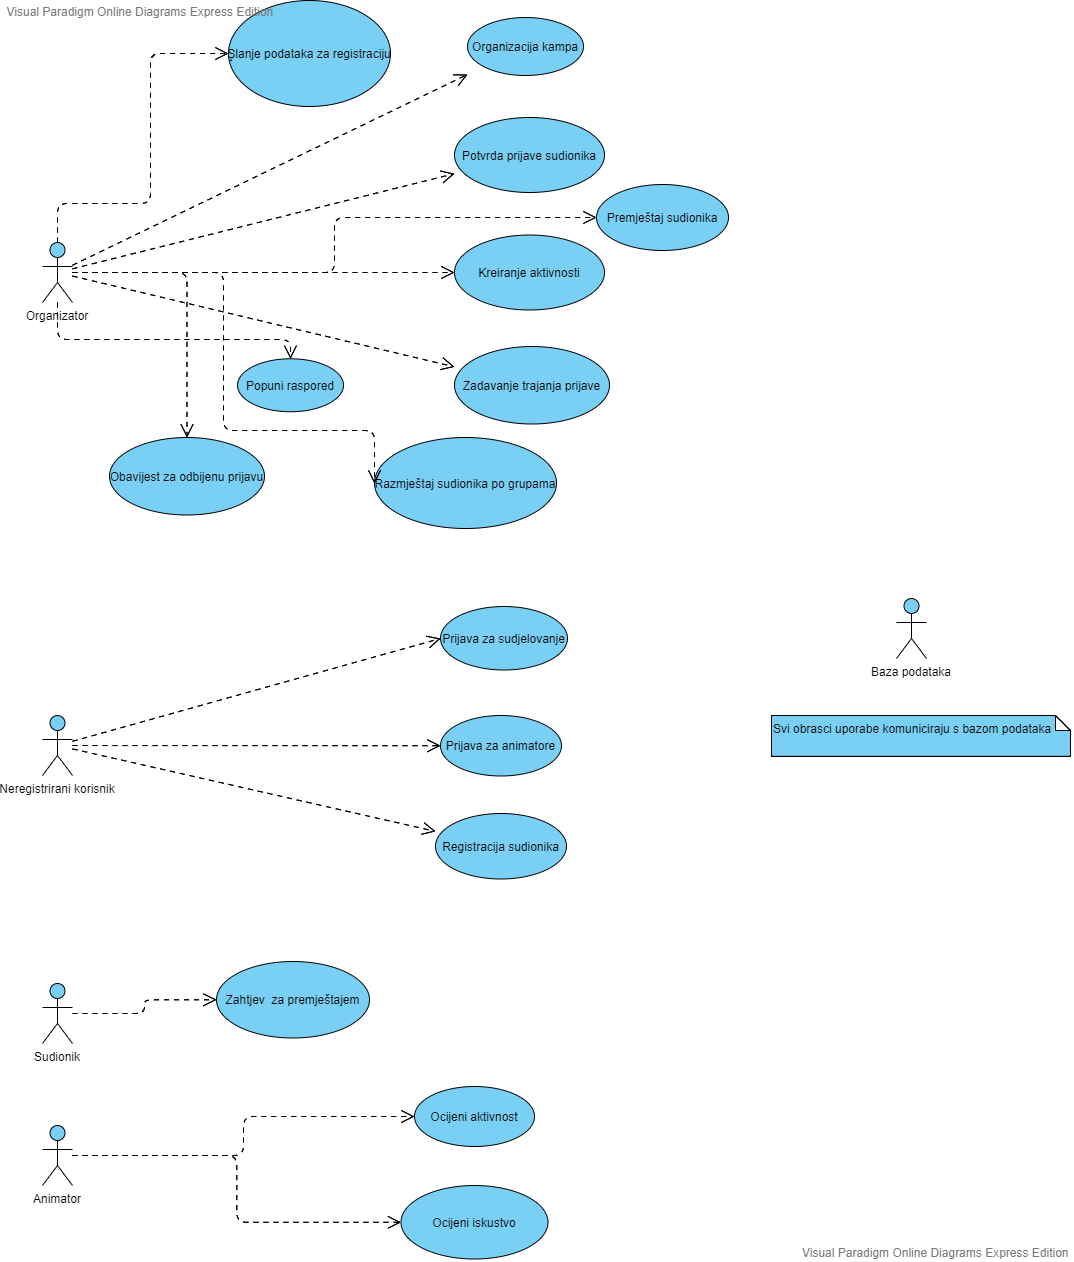
\includegraphics[scale=0.45]{dijagrami/dijagramObrazacaUporabe.PNG}
	\caption{Dijagram obrazaca uporabe}
\end{figure}
\newpage

\subsection{Sekvencijski dijagrami}\label{sec:sekvencijski-dijagrami}
\textbf{Obrazac upotrebe UC1 - Organizacija kampa}\\
\begin{figure}[H]
	\centering
	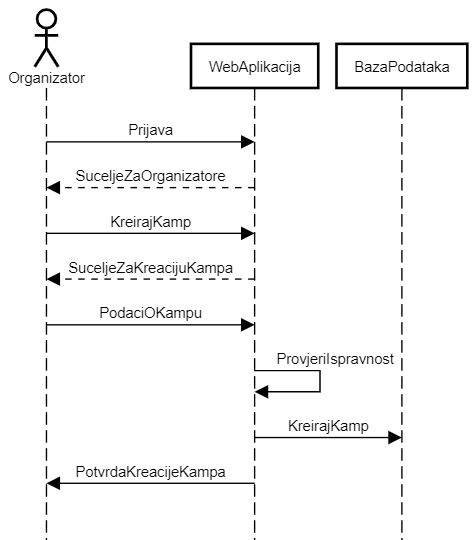
\includegraphics[scale=0.6]{dijagrami/UC1.PNG}
	\caption{Sekvencijski dijagram za UC1}
	\label{fig: uc1 sekv}
\end{figure}

%===========================================================
\newpage
\textbf{Obrazac upotrebe UC2 - Kreiranje aktivnosti}
\begin{figure}[H]
	\centering
	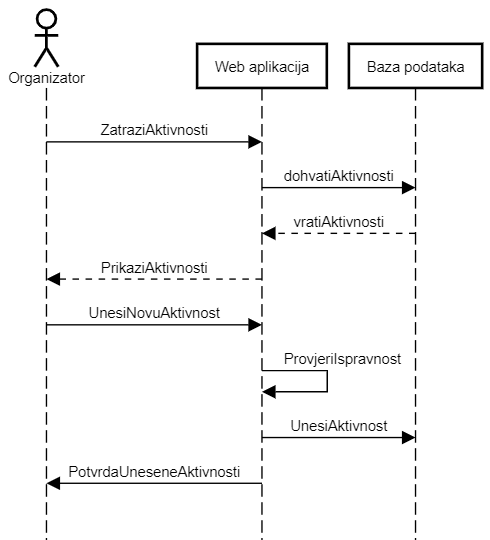
\includegraphics[scale=0.6]{dijagrami/UC2.PNG}
	\caption{Sekvencijski dijagram za UC2}
	\label{fig: uc2 sekv}
	\label{fig: uc2 sekv}
\end{figure}

%===========================================================
\newpage
\textbf{Obrazac upotrebe UC3 - Zadavanje trajanja prijave}
\begin{figure}[H]
	\centering
	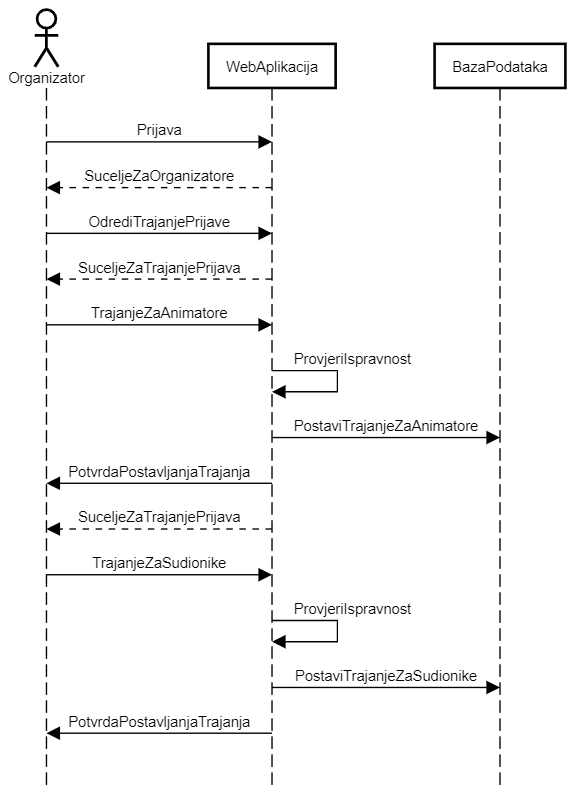
\includegraphics[scale=0.6]{dijagrami/UC3.PNG}
	\caption{Sekvencijski dijagram za UC3}
	\label{fig: uc3 sekv}
\end{figure}


%===========================================================
\newpage
\textbf{Obrazac upotrebe UC4 - Prijava za sudjelovanje}
\begin{figure}[H]
	\centering
	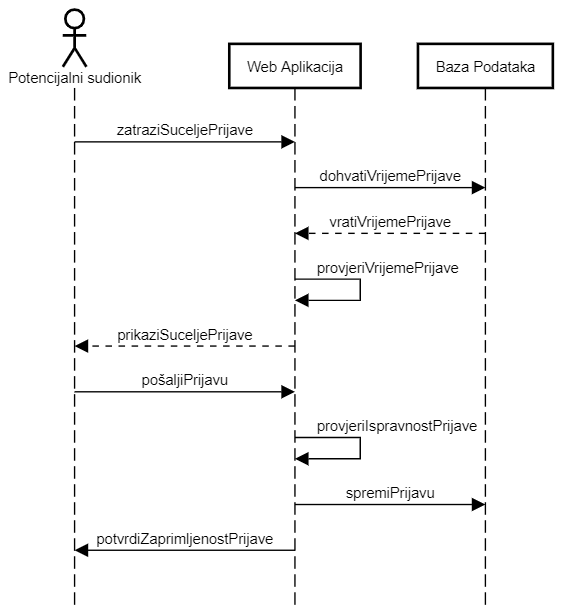
\includegraphics[scale=0.6]{dijagrami/UC4.PNG}
	\caption{Sekvencijski dijagram za UC4}
	\label{fig: uc4 sekv}
\end{figure}


\newpage
\section{Ostali zahtjevi}
\begin{itemize}
	\item sustav treba biti implementiran kao web aplikacija koristeći objektno-orijentirane jezike
	\item korisničko sučelje i sustav moraju podržavati hrvatsku abecedu (dijakritičke znakove) pri unosu i prikazu tekstualnog sadržaja
	\item nadogradnja sustava ne smije narušavati postojeće funkcionalnosti sustava
	\item neispravno korištenje korisničkog sučelja ne smije narušiti funkcionalnost i rad sustava
	\item sustav treba biti jednostavan za korištenje, korisnici se moraju znati koristiti sučeljem bez opširnih uputa
	\item sustav treba omogućiti rad više korisnika u stvarnom vremenu
	\item izvršavanje dijela programa u kojem se pristupa bazi podataka ne smije trajati duže od nekoliko sekundi
	\item pristup sustavu mora biti omogućen iz javne mreže
\end{itemize}
	\chapter{Arhitektura i dizajn sustava}
Arhitektura se može podijeliti na tri podsustava:
\begin{packed_item}
	\item web poslužitelj
	\item web aplikacija
	\item baza podataka
\end{packed_item}
\underbar{Web preglednik} je program koji korisniku omogućuje pregled web-stranica i multimedijalnih sadržaja vezanih uz njih. Svaka stranica pisana je u kodu, a web preglednik je pretvara u ono što mi vidimo. Dakle, svaki internetski preglednik je
prevoditelj. Korisnik putem web preglednika šalje zahtjev web poslužitelju.
\newline \underbar{Web poslužitelj} osnova je rada web aplikacije. On šalje i prima podatke od mnogostrukih klijenata. Komunikacija između njega i korisnika se odvija preko HTTP (engl. Hyper Text Transfer Protocol) protokola, što je protokol u prijenosu informacija na webu. Poslužitelj je onaj koji pokreće web aplikaciju te joj prosljeđuje
zahtjev.
\newline Za obrađivanje željenih zahtjeva koristi se \underbar{web aplikacija}. Ako je potrebno pristupa
bazi podataka te preko poslužitelja korisniku vraća odgovor u obliku HTML dokumenta vidljivog u web pregledniku.
\newline Programski jezik koji smo odabrali za izradu naše web aplikacije je JavaScript zajedno
sa Bootstrap radnim okvirom te HTML i CSS programske jezike za oblikovanje.
Odabrano razvojno okruženje programske potpore je Visual studio code.
\newline Temelj arhitekture sustava ležat će na MVC (Model-View-Controller) konceptu. Naime, taj koncept ima već napravljene predloške koji nam pomažu u izradi web aplikacije te je podržan od radnog okvira. Velika prednost MVC koncepta je da omogućuje programeru da razvija komponente aplikacije nezavisno jedne o drugima,
što olakšava testiranje, traženje grešaka i dodavanje novih funkcionalnosti.
\newline MVC koncept sastoji se od 3 dijela:
\begin{packed_item}
	\item Model – centralni dio sustava koji direktno upravlja podacima, logikom i pravilima sustava. Isto tako prima ulazne podatke Controllera
	\item View – glavna uloga mu je da prikazuje podatke. Ista informacija može se prikazati na nekoliko različitih načina, poput grafova, tablica i sl.
	\item Controller – bavi se prilagodavanjem ulaza koje prosljeduje Modelu i Viewu te upravlja zahtjevima korisnika i pomoću njih djeluje na ostale sustave.
\end{packed_item}

		
		\section{Baza podataka}
			
Za potrebe našeg sustava za organizaciju kampa računarstva „Mlade nade” koristimo relacijsku bazu podataka. Relacijska baza sastoji se od relacija, tj. tablica koje sadrže naziv i skup atributa. Ovakva baza nam omogućuje brzu i jednostavnu pohranu i izmjenu podataka te dohvat podataka za daljnju obradu. Dijagram baze olakšava razumijevanje namjene podataka i njihove povezanosti.\\
Baza podataka ove aplikacije sastoji se od sljedećih entiteta:
\begin{packed_item}
	\item Osoba
	\begin{packed_item}
		\item Animator
		\item Sudionik
		\item Organizator
	\end{packed_item}
	\item Aktivnost
	\begin{packed_item}
		\item Aktivnost1
		\item AktivnostSve
		\item AktivnostMaxN
		\item AktivnostN
	\end{packed_item}
	\item Grupa
	\item Sudjeluje
	\item Račun
	\item Dojam
	\item Prijava
	\item Kamp
\end{packed_item} 
\subsection {Opis tablica}
\textit {\textbf{osoba -}} ovaj entitet sadrži podatke o osobama koje na bilo koji način sudjeluju u kampu. Sadrži atribute: puno ime osobe, ID osobe, motivacijsko pismo, datum rođenja, broj telefona odgovorne osobe (za sudionike mlađe od 18 godina), e-mail i broj telefona. Generalizacija je entiteta organizator, animator i sudionik. U vezi je one-to-one s entitetom dojam preko atributa Idosobe.
\\
\definecolor{aquamarine}{rgb}{0.5, 1.0, 0.83}
\definecolor{blizzardblue}{rgb}{0.67, 0.9, 0.93}
\begin{tabular} {|l|l|l|}
	
	\hline \multicolumn{3}{|c|}{\textbf{osoba}}	 \\ \hline
	
	\cellcolor{aquamarine}Idosobe & INT	&  	identifikacijski broj osobe\\ \hline
	punoIme	& VARCHAR &   ime i prezime osobe	\\ \hline 
	motPismo & VARCHAR &  motivacijsko pismo \\ \hline 
	datumRod & DATE	&  	datum rođenja osobe	\\ \hline 
	brojTelefonaOdgOsobe & 	VARCHAR	&	broj telefona odgovorne osobe \\ \hline
	Email &	VARCHAR	&	e-mail osobe \\ \hline
	brojTel	&	VARCHAR	&	broj telefona osobe \\ \hline
\end{tabular}\\
\\
\\
\textbf{\textit{animator -}} ovaj entitet sadrži podatke o animatorima koji sudjeluju u raznim aktivnostima. Specijalizacija je entiteta osoba. Uz atribute entiteta osoba sadrži još i entitet naziv aktivnosti. U vezi je many-to-one s entitetom aktivnost preko atributa nazivAkt.\\
\begin{tabular}{|l|l|l|}
	
	\hline \multicolumn{3}{|c|}{\textbf{animator}}	\\  \hline
	
	\cellcolor{aquamarine}Idosobe & INT	&  	identifikacijski broj osobe\\ \hline
	\cellcolor{blizzardblue}nazivAkt	& VARCHAR &   naziv aktivnosti u kojoj sudjeluje	\\ \hline 
	punoIme	& VARCHAR &   ime i prezime osobe	\\ \hline 
	motPismo & VARCHAR &  motivacijsko pismo \\ \hline 
	datumRod & DATE	&  	datum rođenja osobe	\\ \hline 
	brojTelefonaOdgOsobe & 	VARCHAR	&	broj telefona odgovorne osobe \\ \hline
	Email &	VARCHAR	&	e-mail osobe \\ \hline
	brojTel	&	VARCHAR	&	broj telefona osobe \\ \hline
\end{tabular} \\ \\
\\
\\
\textbf{\textit{sudionik -}} ovaj entitet sadrži podatke o sudionicima kampa. Specijalizacija je entiteta osoba. Uz atribute entiteta osoba sadrži još i entitet naziv grupe. U vezi je many-to-one s entitetom grupa preko atributa nazivGrupa.\\
\begin{tabular}{|l|l|l|}
	
	\hline \multicolumn{3}{|c|}{\textbf{Sudionik}}\\ \hline
	
	\cellcolor{aquamarine}Idosobe & INT	&  	identifikacijski broj osobe\\ \hline
	\cellcolor{blizzardblue}nazivGrupa	& VARCHAR &   naziv grupe čiji je član	\\ \hline 
	punoIme	& VARCHAR &   ime i prezime osobe	\\ \hline 
	motPismo & VARCHAR &  motivacijsko pismo \\ \hline 
	datumRod & DATE	&  	datum rođenja osobe	\\ \hline 
	brojTelefonaOdgOsobe & 	VARCHAR	&	broj telefona odgovorne osobe \\ \hline
	Email &	VARCHAR	&	e-mail osobe \\ \hline
	brojTel	&	VARCHAR	&	broj telefona osobe \\ \hline
\end{tabular} \\ \\
\\
\textbf{\textit{organizator -}} ovaj entitet sadrži informacije o osobi koja organizira kamp. Specijalizacija je entiteta osoba. Uz atribute entiteta osoba sadrži još i entitet nazivGrupa.\\
\begin{tabular}{|l|l|l|}
	
	\hline \multicolumn{3}{|c|}{\textbf{organizator}}\\	 \hline
	
	\cellcolor{aquamarine}Idorganizatora & INT	&  	identifikacijski broj organizatora\\ \hline
	punoIme	& VARCHAR &   ime i prezime osobe	\\ \hline 
	motPismo & VARCHAR &  motivacijsko pismo \\ \hline 
	datumRod & DATE	&  	datum rođenja osobe	\\ \hline 
	brojTelefonaOdgOsobe & 	VARCHAR	&	broj telefona odgovorne osobe \\ \hline
	Email &	VARCHAR	&	e-mail osobe \\ \hline
	brojTel	&	VARCHAR	&	broj telefona osobe \\ \hline 
\end{tabular} \\ \\
\\
\textbf{\textit{aktivnost -}} ovaj entitet sadrži podatke o aktivnostima koje se odvijaju u kampu. Generalizacija je entiteta aktivnost1, aktivnostSve, aktivnostMaxN i aktivnostN. Sadrži atribute naziv aktivnosti, opis i trajanje aktivnosti. U vezi je many-to-one s entitetom sudjeluje preko atributa nazivAkt. \\
\begin{tabular}{|l|l|l|}
	
	\hline \multicolumn{3}{|c|}{\textbf{aktivnost}}	\\ \hline
	
	\cellcolor{aquamarine}nazivAkt & VARCHAR &  Naziv aktivnosti\\ \hline 
	opis &	VARCHAR	& Kratak opis aktivnosti\\ \hline
	trajanje & INTERVAL & Trajanje aktivnosti\\ \hline
\end{tabular} \\ \\
\\
\textbf{\textit{aktivnost1 -}} ovaj entitet sadrži podatke o aktivnostima u kojima sudjeluje samo jedna grupa sudionika. Specijalizacija je entiteta aktivnost. Sadrži sve atribute entiteta aktivnost tj. naziv aktivnosti, opis i trajanje.\\
\begin{tabular}{|l|l|l|l|}
	
	\hline \multicolumn{3}{|c|}{\textbf{aktivnost1}}\\ \hline
	
	\cellcolor{aquamarine}nazivAkt & VARCHAR	&  	naziv aktivnosti\\ \hline 
	opis	&	VARCHAR	&	kratak opis aktivnosti\\ \hline
	trajanje & INTERVAL & trajanje aktivnosti\\ \hline
\end{tabular} \\ \\
\\
\textit{\textbf{aktivnostSve -}} ovaj entitet sadrži podatke o aktivnostima u kojima sudjeluju sve postojeće grupe sudionika. Specijalizacija je entiteta aktivnost. Sadrži sve atribute entiteta aktivnost tj. naziv aktivnosti opis i trajanje.\\
\begin{tabular}{|l|l|l|l|}
	
	\hline \multicolumn{3}{|c|}{\textbf{aktivnostSve}}	\\  \hline
	
	\cellcolor{aquamarine}nazivAkt & VARCHAR	&  	naziv aktivnosti\\ \hline 
	opis	&	VARCHAR	&	kratak opis aktivnosti\\ \hline
	trajanje & INTERVAL & trajanje aktivnosti\\ \hline
\end{tabular} \\ \\
\\
\textbf{\textit{aktivnostMaxN -}} ovaj entitet sadrži podatke o aktivnostima u kojima sudjeluje maksimalno N grupa sudionika. Specijalizacija je entiteta aktivnost. Sadrži sve atribute entiteta aktivnost tj. naziv aktivnosti, opis i trajanje.\\
\begin{tabular}{|l|l|l|l|}
	
	\hline \multicolumn{3}{|c|}{\textbf{aktivnostMaxN}}	\\  \hline
	
	\cellcolor{aquamarine}nazivAkt & VARCHAR	&  	naziv aktivnosti\\ \hline
	opis	&	VARCHAR	&	kratak opis aktivnosti\\ \hline
	trajanje & INTERVAL & trajanje aktivnosti\\ \hline 
\end{tabular} \\ \\
\\
\textbf{\textit{aktivnostN -}} ovaj entitet  sadrži podatke o aktivnostima u kojima sudjeluje točno N grupa sudionika. Specijalizacija je entiteta aktivnost. Sadrži sve atribute entiteta aktivnost tj. naziv aktivnosti, opis i trajanje.\\
\begin{tabular}{|l|l|l|l|}
	
	\hline \multicolumn{3}{|c|}{\textbf{aktivnostN}}\\	 \hline
	
	\cellcolor{aquamarine}nazivAkt & VARCHAR	&  	naziv aktivnosti\\ \hline
	opis	&	VARCHAR	&	kratak opis aktivnosti\\ \hline
	trajanje & INTERVAL & trajanje aktivnosti\\ \hline 
\end{tabular} \\ \\
\\
\textbf{\textit{grupa -}} ovaj entitet opisuje grupe sudionika koji sudjeluju u aktivnostima. Sadrži atribut naziv grupe. U vezi je many-to-one s entitetom sudjeluje preko atributa nazivGrupa. \\
\begin{tabular}{|l|l|l|l|}
	
	\hline \multicolumn{3}{|c|}{\textbf{grupa}}	\\  \hline
	
	\cellcolor{aquamarine}nazivGrupa & VARCHAR	&  	naziv grupe sudionika\\ \hline 
\end{tabular} \\ \\
\\
\textbf{\textit{sudjeluje -}} ovaj entitet sadrži sve informacije o odnosu grupa i aktivnosti, odnosno daje informacije o tome koja grupa sudjeluje u kojoj od aktivnosti. Sadrži atribut naziv grupe te je preko tog atributa u vezi one-to-many s entitetom sudionik.\\
\begin{tabular}{|l|l|l|l|}
	
	\hline \multicolumn{3}{|c|}{\textbf{sudjeluje}}\\	  \hline
	
	\cellcolor{aquamarine}nazivGrupa & VARCHAR	&  	naziv grupe sudionika\\ \hline 
	\cellcolor{aquamarine} nazivAkt	&	VARCHAR	&	naziv aktivnosti\\ \hline
\end{tabular} \\ \\
\\
\textbf{\textit{račun -}} ovaj entitet sadrži podatke o korisničkom računu koji je se izrađuje na temelju prihvaćene prijave za svakog sudionika i animatora. Sadrži atribute korisnickoIme, lozinka, poveznica i Idosobe. U vezi je one-to-one s entitetom osoba preko atributa Idosobe. \\
\begin{tabular}{|l|l|l|l|}
	
	\hline \multicolumn{3}{|c|}{\textbf{račun}}	\\  \hline
	
	\cellcolor{aquamarine}korisnickoIme & VARCHAR	&  	korisničko ime osobe\\ \hline 
	\cellcolor{blizzardblue} Idosobe	&	INT	&	identifikacijski broj osobe\\ \hline
	lozinka	&	VARCHAR	&	lozinka korisničkog računa\\ \hline
	poveznica	&	VARCHAR	&	poveznica za registraciju\\ \hline
\end{tabular} \\ \\
\\
\textbf{\textit{dojam -}} ovaj entitet sadrži informacije o osvrtu i ocjeni koju sudionici i animatori ostavljaju nakon završetka kampa. Sadrži entitete ID osobe, ocjena, komentar. U vezi je one-to-one s entitetom osoba preko atributa Idosobe.\\
\begin{tabular}{|l|l|l|l|}
	
	\hline \multicolumn{3}{|c|}{\textbf{dojam}}	\\  \hline
	
	\cellcolor{aquamarine}Idosobe	&	INT	&	identifikacijski broj osobe\\ \hline
	ocjena	&	INT	&	ocjena kampa\\ \hline
	komentar	&	VARCHAR	&	kratki osvrt\\ \hline
\end{tabular} \\ \\
\\
\textbf{\textit{prijava -}} ovaj entitet sadrži podatke o prijavama za sudjelovanje u kampu. Sadrži atribute prijavaZa (određuje prijavljuje li se osoba za sudionika ili animatora), vrijeme početka prijave i vrijeme trajanja prijave. \\
\begin{tabular}{|l|l|l|l|}
	
	\hline \multicolumn{3}{|c|}{\textbf{prijava}}\\	\hline
	
	prijavaZa	&	VARCHAR	&	prijava za sudionika/animatora\\ \hline
	vrijemePocetka	&	TIMESTAMP	&	vrijeme početka prijave\\ \hline
	vrijemeTrajanja	&	INTERVAL	&	trajanje prijave\\ \hline
\end{tabular} \\ \\
\\
\textbf{\textit{kamp -}} ovaj enitet sadrži informacije o kampu za računarstvo za koji se izrađuje aplikacija. Sadrži atribute vrijemePocetka i vrijemeTrajanje.\\
\begin{tabular}{|l|l|l|l|}
	
	\hline \multicolumn{3}{|c|}{\textbf{kamp}}\\	  \hline
	
	vrijemePocetka	&	TIMESTAMP	&	vrijeme početka kampa\\ \hline
	vrijemeTrajanja	&	INTERVAL	&	trajanje kampa\\ \hline
\end{tabular} \\ \\


			
			
			\subsection{Dijagram baze podataka}
\vspace {10pt} \textbf {Dijagram baze podataka}\\
\begin{figure}[htb]
	\centering
	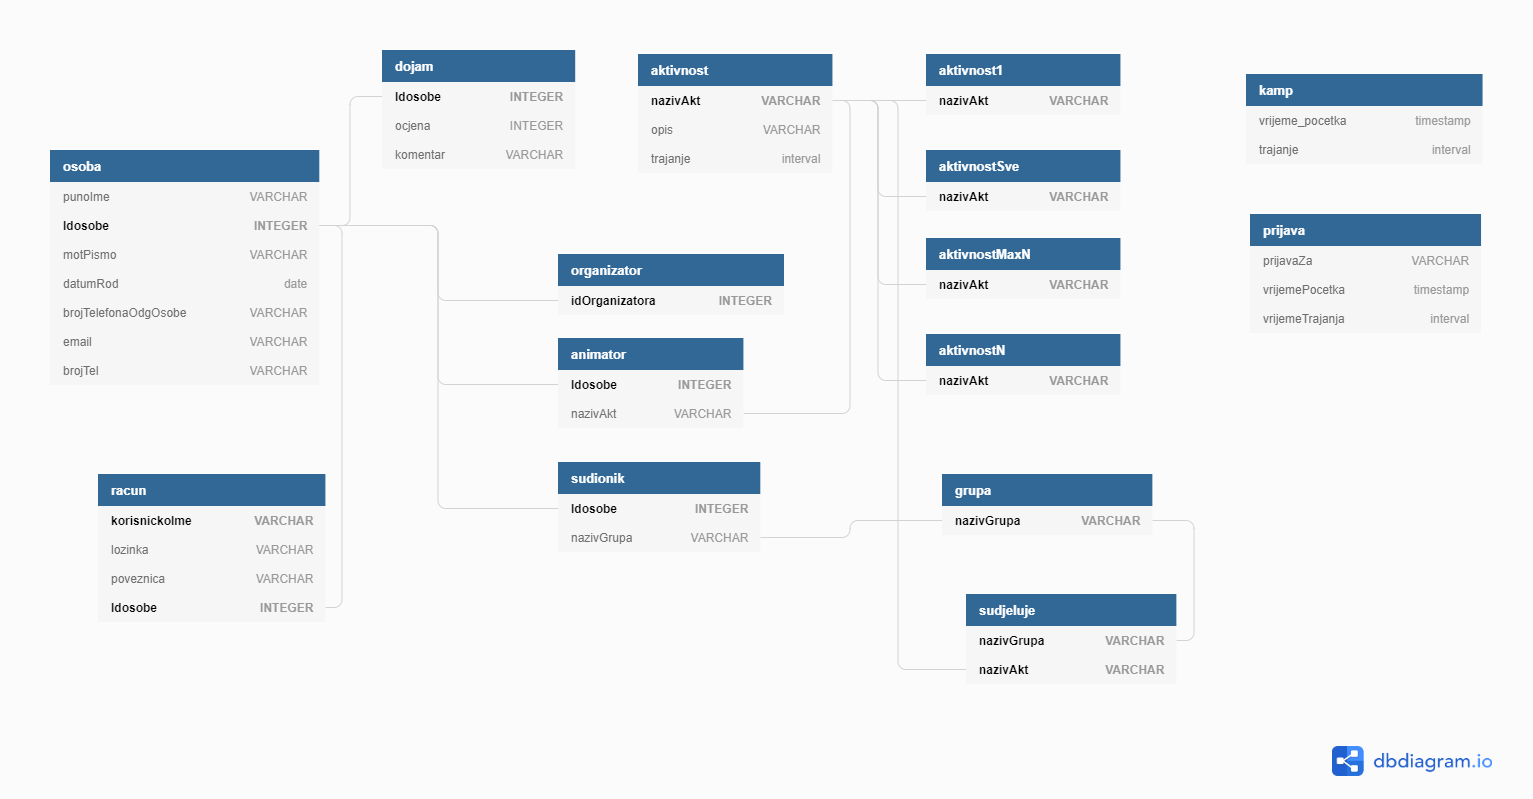
\includegraphics[scale=0.25]{dijagrami/dataBase.PNG}
	\caption{ER dijagram baze podataka}
	\label{fig: dijagram baze}
\end{figure}
			
			\eject
			
			\newpage
			
		\section{Dijagram razreda}
		
Na slikama 4.2 i 4.3 prikazani su razredi koji pripadaju backend dijelu MVCarhitekture.  Razredi prikazani na slici 4.2 nasljeduju Controller razred.  Metode implementirane u tim razredima manipuliraju s podacima, a oni su dohvaćeni pomoću metoda implementiranih u Model razredima.  Metode implementirane u Controller razredima vraćaju JSON datoteke s html status kodom. Prikazane su samo ovisnosti između razreda koji pripadaju istom dijelu dijagrama. Iz naziva i tipova atributa u razredima možemo zaključiti vrstu ovisnosti među različitim razredima. \\
\begin{figure}[htpb]
	\centering
	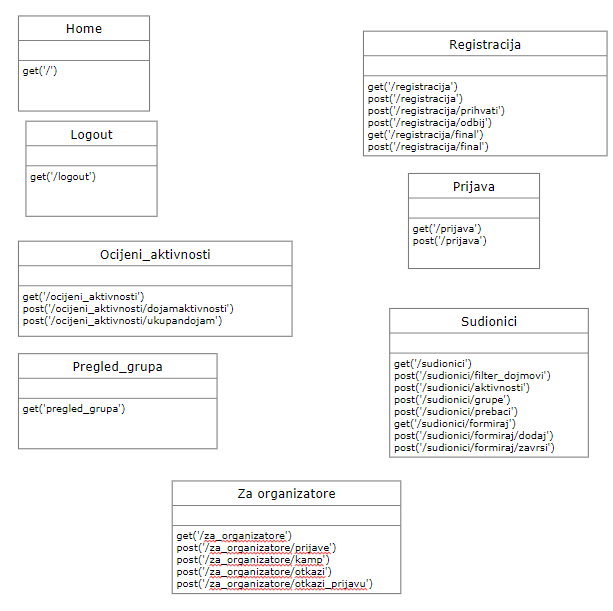
\includegraphics[scale=1]{dijagrami/controller_uml.PNG}
	\caption{Dijagram razreda - dio Controllers}
	\label{fig: dijagram razreda models}
\end{figure}
\newpage

Model razredi preslikavaju strukturu baze podataka u aplikaciji. Metode koje su implementirane direktno komuniciraju s bazom podataka i tako vraćaju tražene podatke. Razred Korisnik predstavlja neregistriranog korisnika koji se može registrirati u sustav unoseći tražene informacije. Također ako je već registriran, može se prijaviti u sustav. Nakon prijave on može biti registriran kao Sudionik ili kao Animator, i ovisno o tome može koristiti drugačije funkcionalnosti stranice. Razred Organizator predstavlja osobu koja može razmještati ostale korisnike po grupama i koja ima najveće ovlasti.\\

\begin{figure}[htpb]
	\centering
	\includegraphics[scale=0.3]{dijagrami/UMLdiagram.PNG}
	\caption{Dijagram razreda - dio Models}
	\label{fig: dijagram razreda models}
\end{figure}
\eject

		\eject
		\newpage
		
		\section{Dijagram stanja}
			
			
Dijagram stanja je dijagram koji prikazuje određena stanja objekata i prijelaze jednog stanja u drugo temeljene na određenim događajima. Na slici 4.4 prikazan je dijagram stanja za prijavu otprije registriranog korisnika – Sudionika i o prikazu njegovih opcija ovisno o tome je li kamp počeo, traje, ili je završio. Nakon prijave, ako kamp još nije počeo sudioniku se prikazuje odbrojavanje do početka kampa i klikom može kontaktirati organizatora. Nakon prijave i nakon početka kampa, sudionik vidi svoj osobni raspored ili agendu, te klikom na \textit{Popis članova} može vidjeti popis članova i njihove kontakte. Naposljetku, nakon prijave i nakon završetka kampa, sudionik može ocijeniti svoje cjelokupno iskustvo i ostaviti dojam.
			
\begin{figure}[htb]
	\centering
	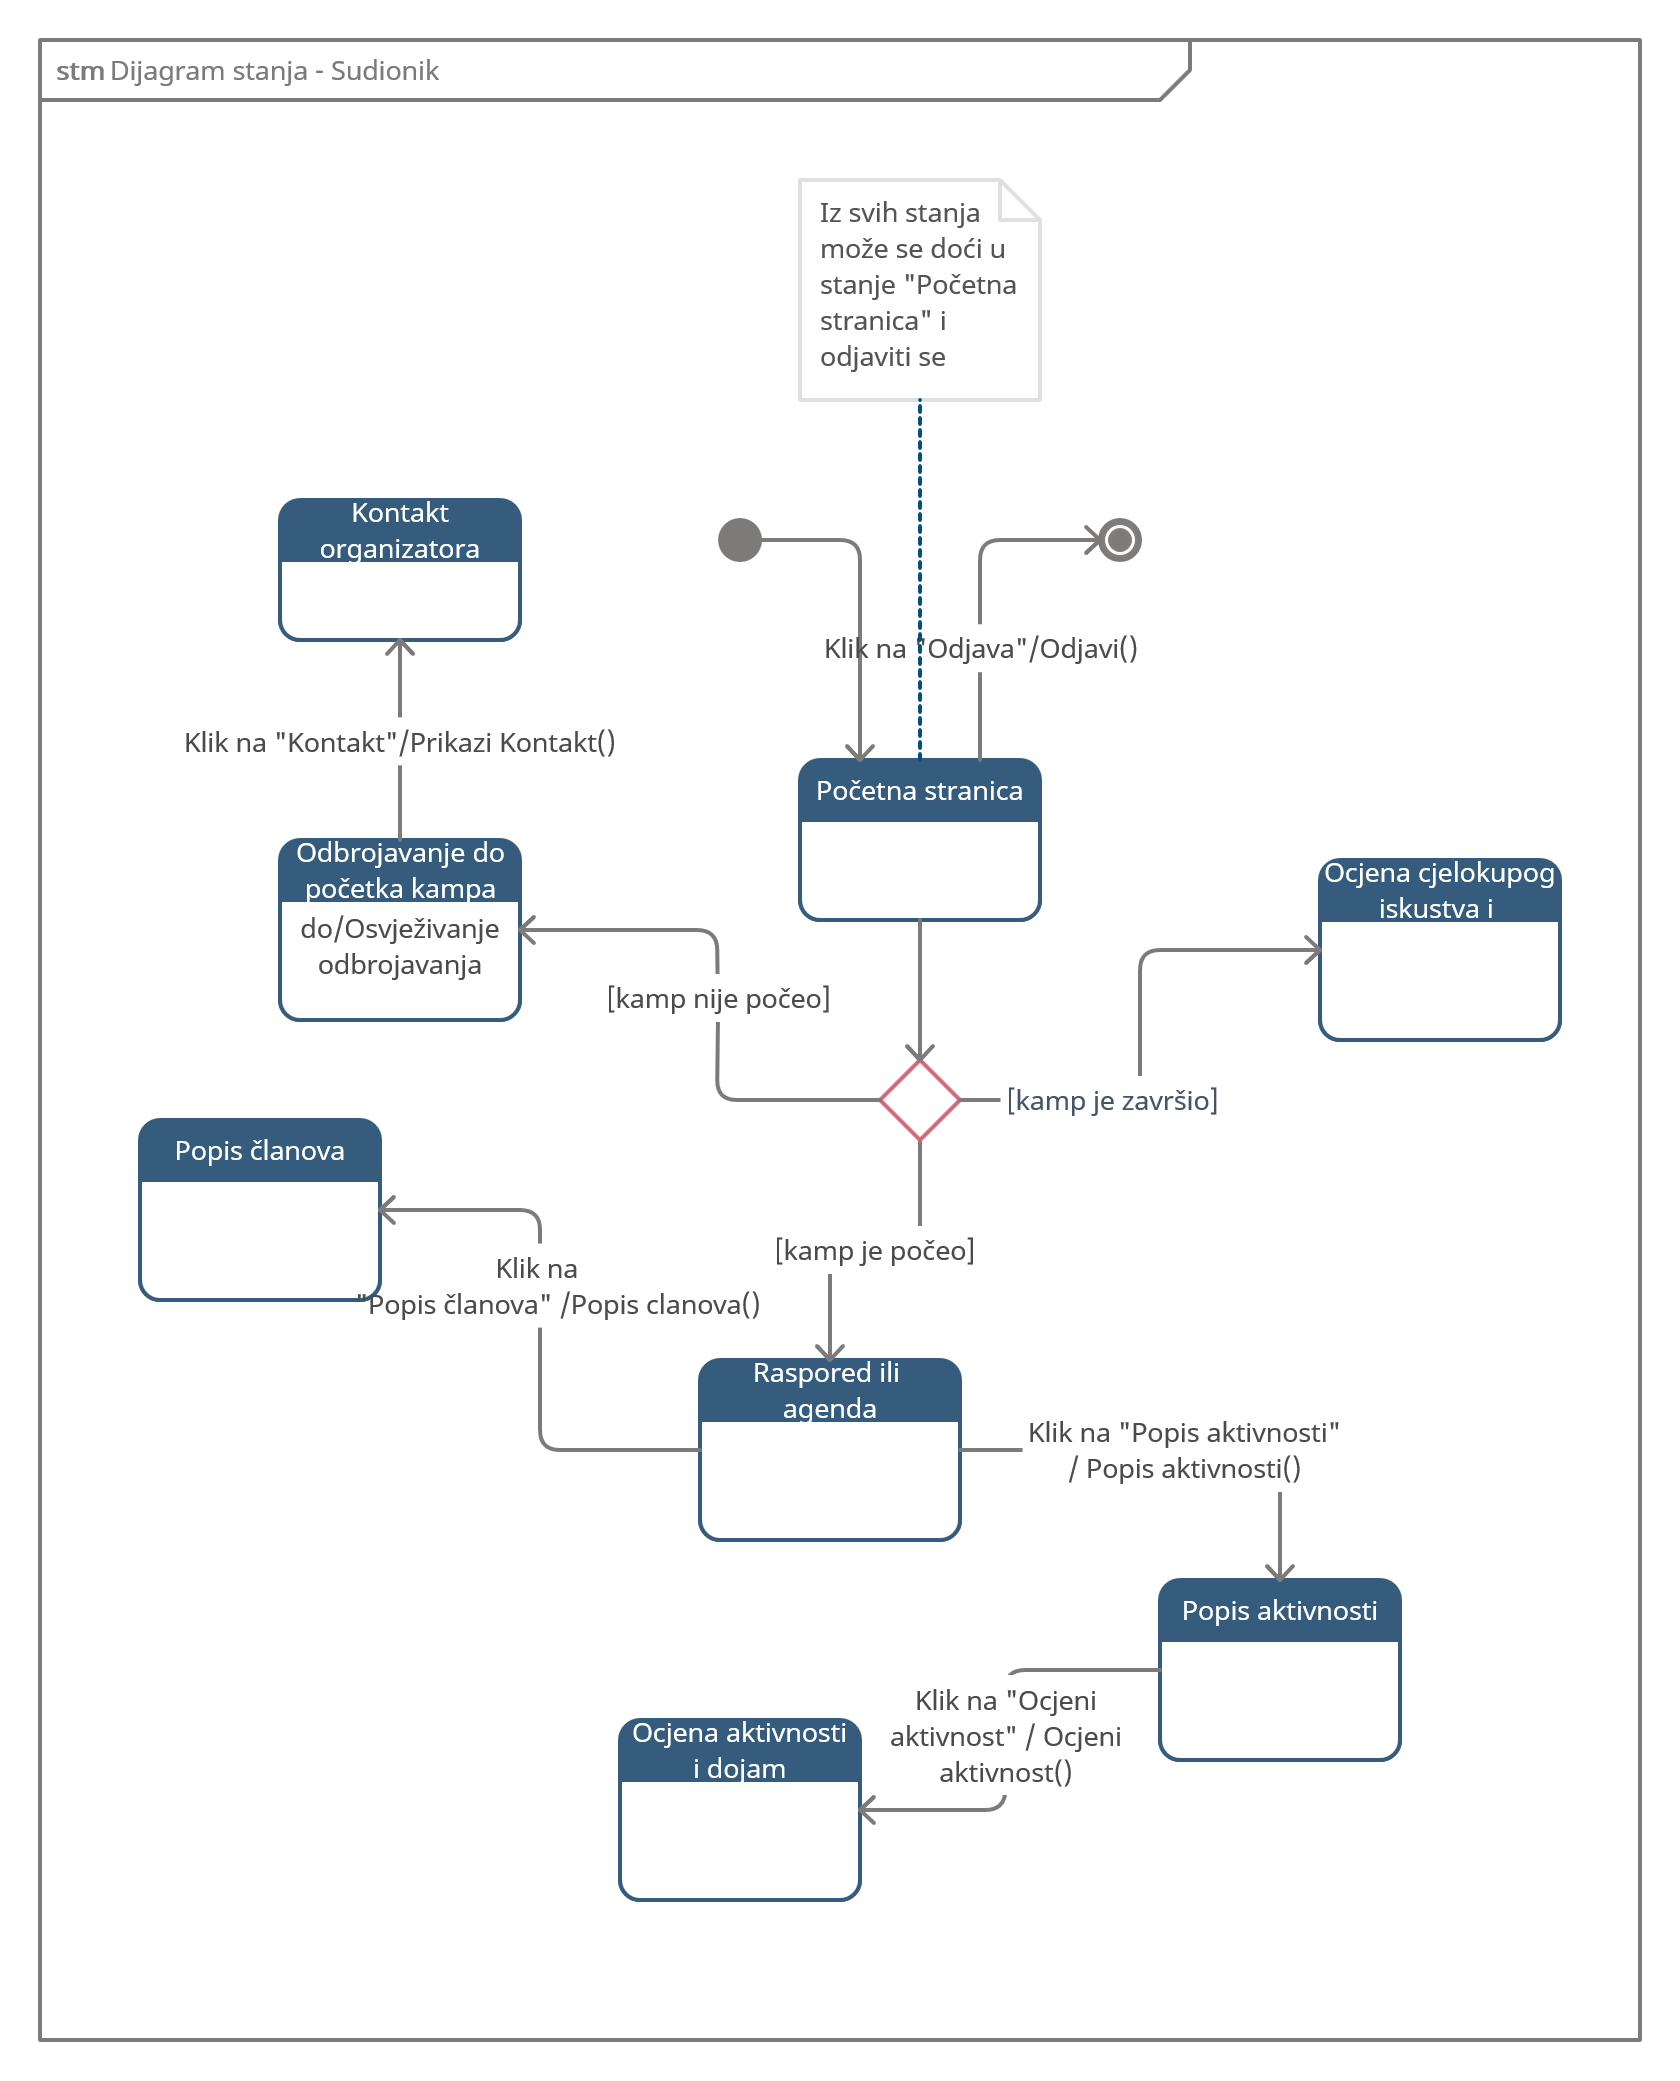
\includegraphics[scale=0.2]{dijagrami/dijagramStanja.PNG}
	\caption{Dijagram stanja}
	\label{fig: dijagram stanja}
\end{figure}
		\eject
		
		\section{Dijagram aktivnosti}
			
Dijagram aktivnosti primjenjuje se za opis modela toka upravljanja ili podatkovnog toka te modeliranje poslovnih procesa. To je u osnovi dijagram toka koji predstavlja tok iz jedne u drugu aktivnost. U modeliranju toka upravljanja svaki novi korak poduzima se nakon završenog prethodnog, a naglasak je na jednostavnosti.
Na slici 4.5 prikazan je proces ostavljanje dojma i ocjene korisnika za određenu aktivnost. Korisnik se prijavi u sustav te s popisa odabere jednu od aktivnosti u kojima sudjeluje. Zatim mu se prikazuje okvir za upis dojma i ocjene. Nakon upisivanja dojma i ocjene, podaci se spremaju u bazu podataka i korisnik se može odjaviti. \\

\begin{figure}[htb]
	\centering
	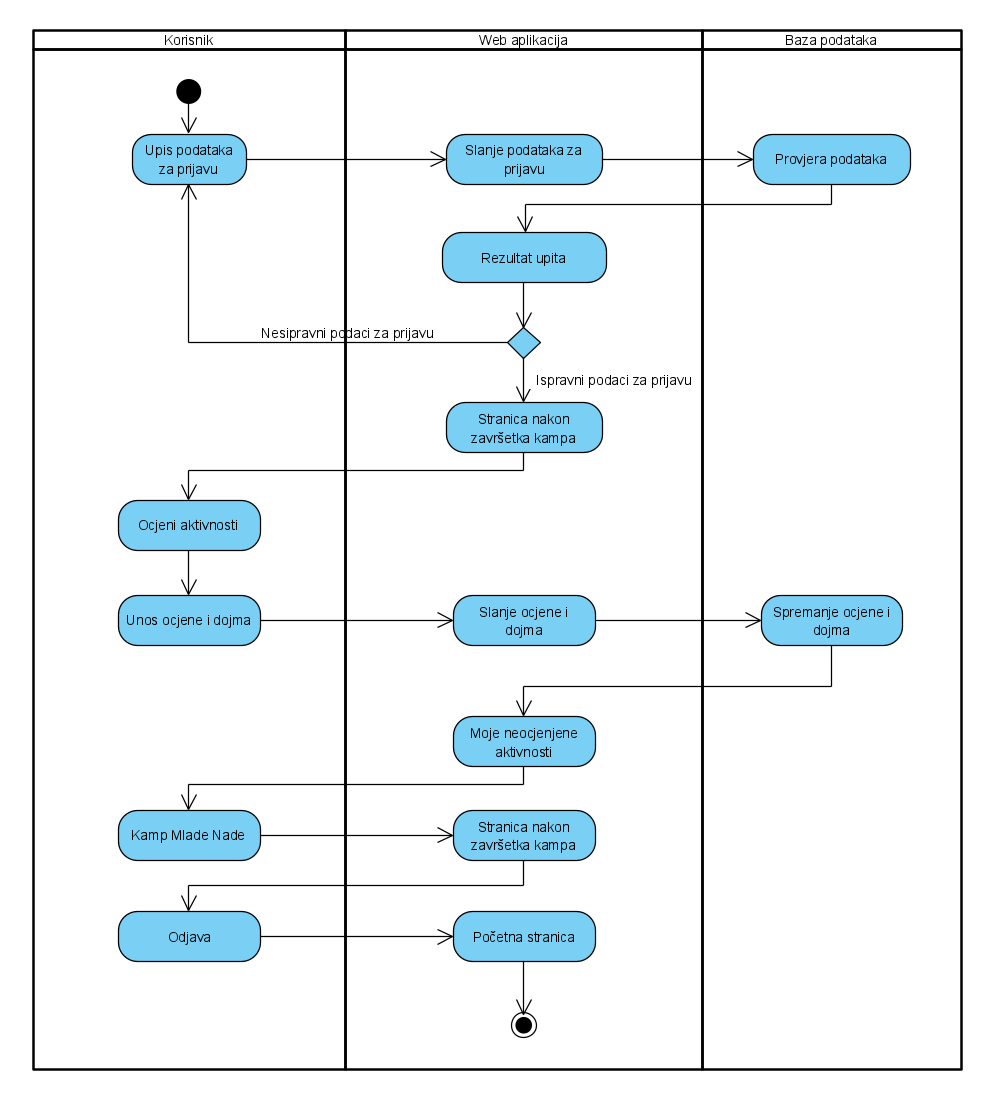
\includegraphics[scale=0.5]{dijagrami/dijagramAktivnosti.PNG}
	\caption{Dijagram aktivnosti}
	\label{fig: dijagram aktivnosti}
\end{figure}

		\eject
		
	\section{Dijagram komponenti}
	
		Sustavu se pristupa putem dva sučelja. Preko sučelja za dohvat HTML, CSS i JS datoteka poslužuju se datoteke koje pripadaju frontendu. Router je komponenta koja na upit s url-om određuje koja će se datoteka poslužiti na sučelje. Frontend se sastoji od niza JavaScript datoteka koje su raspoređene u simboličke cjeline i ovise o React biblioteci iz koje dohvaćaju gotove komponente (gumbi, forme i sl.). Backend je baziran na arhitekturi \textit{Repository Service Controller}. Preko
		sučelja za dohvat JSON podataka pristupa se REST API komponenti. REST API poslužuje podatke koji pripadaju backendu. Razredi koji implementiraju sučelje Service zaduženi su za dohvaćanje podataka iz baze podataka pomoću SQL upita uz pomoć Repositoryja. Podaci koji su pristigli iz baze šalju se MVC arhitekturi u obliku DTO (Data transfer object). React-view komponenta preko dostupnih sučelja komunicira s web aplikacijom te osvježava prikaz i dohvaća nove podatke.
		\begin{figure}[htb]
			\centering
			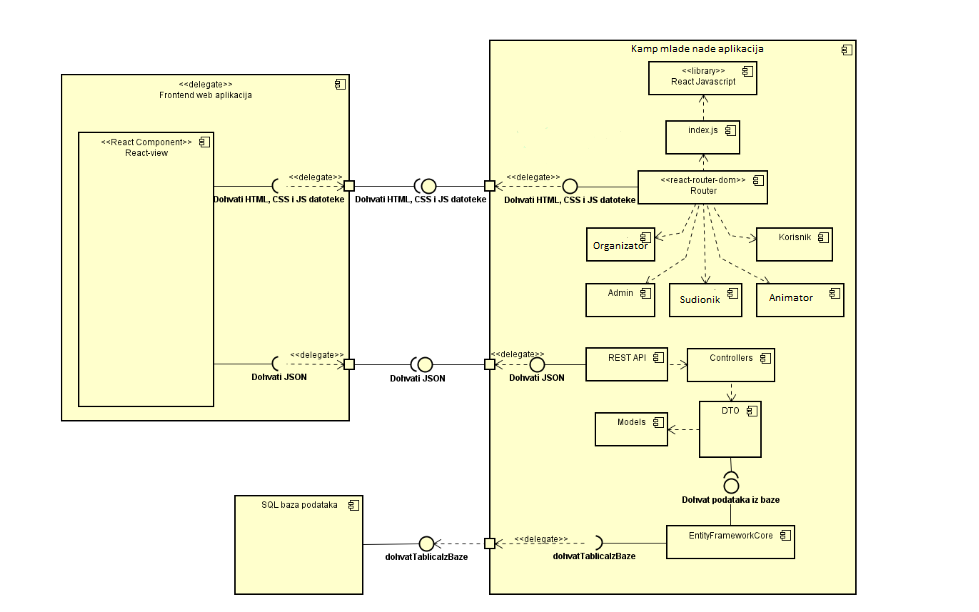
\includegraphics[scale=0.54]{dijagrami/dijagramKomponenti.PNG}
			\caption{Dijagram komponenti}
			\label{fig: dijagram komponenti}
		\end{figure}
			\eject
	
\chapter{Implementacija i korisničko sučelje}

		
		\section{Korištene tehnologije i alati}
		
Komunikacija u timu realizirana je korištenjem aplikacije MS Teams\footnote{\url{https://www.microsoft.com/hr-hr/microsoft-365/microsoft-teams}}.\newline
\indent Za izradu UML dijagrama korišten je alat Visual Paradigm Online\footnote{\url{https://online.visual-paradigm.com}}, a kao sustav za upravljanje izvornim kodom Git\footnote{\url{https://git-scm.com}}, a udaljeni repozitorij projekta je dostupan na web platformi GitLab\footnote{\url{https://gitlab.com/}}.\newline
\indent Kao razvojno okruženje korišten je Visual Studio  Code\footnote{\url{https://code.visualstudio.com/}}, integrirano razvojno okruženje (kratica IDE) tvrtke Microsoft. Koristi se prvenstveno za razvoj računalnih programa za operacijski sustav Windows, kao i za web-stranice, web-aplikacjie, mobilne aplikacije i web-usluge. Visual studio za razvoj softvera koristi Microsoftove platforme kao što su Windows API, Windows Forms, Windows Presentation Foundation, Windows Store i Microsoft Silverlight.\newline
\indent Baza podataka se nalazi na pgAdmin 4 platformi\footnote{\url{https://www.pgadmin.org/}}.\\
			
			\eject 
		
	
		\section{Ispitivanje programskog rješenja}
	
			
			\subsection{Ispitivanje komponenti}
			{U okviru paketa \textbf{Mocha} i \textbf{Chai} proveden je unit testing. Testovi su provedeni nad nekim funkcionalnostima razreda Grupa, Kamp, Sudionik, MailSender i Osoba.\\\\}
			
			\textbf{\large Testovi kamp klase}
			\begin{verbatim}
			const assert = require('assert');
			const Kamp = require('../models/Kamp');
			
			describe('Kamp Test', () => {
				it('treba vratiti undefined jer nema kampa', () => {
					assert.equal(undefined, Kamp.provjeriImaLiKampa().pocetak);
				});
				
				it('treba vratiti 2',async () => {
					let kamp = new Kamp("2021-01-14T18:47", 2, []);
					await kamp.persist();
					let result = await Kamp.provjeriImaLiKampa();
					assert.equal(result.trajanje, 2);
					await Kamp.otkaziKamp();
				});
			});
			\end{verbatim}
		
			\newpage
			
			
			\textbf{\large Testovi grupa}
			\begin{verbatim}
			const assert = require('assert');
			const Grupa = require('../models/Grupa');
			
			describe('Grupa Test', () => {
				it('treba vratiti naziv grupe', async () => {
					let grupa = new Grupa("grupa 1")
					await grupa.persist();
					let result = await Grupa.fetchAllGroups();
					assert.equal(result[0].naziv, "grupa 1");
				});
			});
			\end{verbatim}
			
			
			\textbf{\large Testovi pošiljatelja mailova}
			\begin{verbatim}
			const assert = require('assert');
			const MailSender = require('../models/MailSender');
			
			describe('Mail Sender Test', () => {
				
				it('treba vratiti poruku prihvaćanja', () => {
					let mailOptions = MailSender.send("korisnik@random.com", "krandom", "accepted");
					assert.equal(mailOptions.subject, 'Čestitamo! Primljeni ste u naš kamp!');
				});
				
				it('treba vratiti poruku odbijanja', () => {
					let mailOptions = MailSender.send("korisnik2@random.com", "krandom2", "denied");
					assert.equal(mailOptions.subject, 'Vaš zahtjev je obijen');
				});
			});
			\end{verbatim}
			
			\newpage
			
			\textbf{\large Test za random raspored sudionika u grupe}
			\begin{verbatim}
			const expect = require('chai').expect;
			const assert = require('assert');
			
			
			describe('Shuffle Test', () => {
				
				it('liste trebaju imati ispremiješane elemente',async () => {
					let array = [1, 2, 1, 2, 3, 3];
					let arrayShuffled = [1, 2, 1, 2, 3, 3];
					arrayShuffled = shuffle(arrayShuffled);
					console.log(array);
					console.log(arrayShuffled);
					assert.notStrictEqual(array, arrayShuffled);
				});
				
				it('liste trebaju imati iste elemente', () => {
					let array = [1, 2, 1, 2, 3, 3];
					let arrayShuffled = [1, 2, 1, 2, 3, 3];
					arrayShuffled = shuffle(arrayShuffled);
					expect(array).to.have.same.members(arrayShuffled);
				});
			});
			
			function shuffle(array) {
				for (var i = array.length - 1; i > 0; i--) {
					var j = Math.floor(Math.random() * (i + 1));
					var temp = array[i];
					array[i] = array[j];
					array[j] = temp;
				}
				return array
			}
			\end{verbatim}
		
			\newpage
			
			\textbf{\large Screenshot pokretanja i uspjeha testova}
			
			\begin{figure}[h]
				\centering
				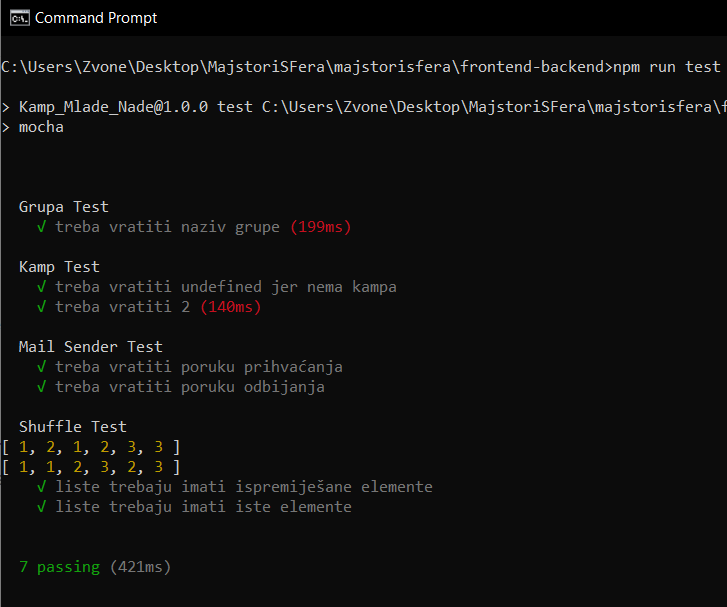
\includegraphics[scale=1.0]{testovi}
				\caption{Pokrenuti testovi}
			\end{figure}
			
			\newpage
			
			\subsection{Ispitivanje sustava}
			
			{Pomoću radnog okvira Selenium provedeno je ispitivanje funkcionalnosti organizacije kampa i organizacije prijave za kamp, prijave osobe na kamp, potvrde prijave od strane organizatora te registracije korisnika. Za izradu ispitnih slučajeva korišten je alat Selenium IDE.\\ }
			
			\textbf{Ispitni slučaj 1: Organizacija kampa i prijava za kamp\\}
				\indent\textbf{Ulaz:}
					\begin{packed_item}
						\item {Prijava kao organizator.}
						\item {Organiziranje kampa u određeno vrijeme.}
						\item {Organiziranje prijava u određeno vrijeme.}
					\end{packed_item}
			
				\textbf{Očekivani rezultat:}
					\begin{packed_item}
						\item {Na početnoj stranici ispisano je vrijeme početka i vrijeme trajanja kampa.}
					\end{packed_item}
			
				{\textbf{Rezultat:} Očekivani rezultat je zadovoljen. Aplikacija je prošla test.}
			
			\begin{figure}[h]
				\centering
				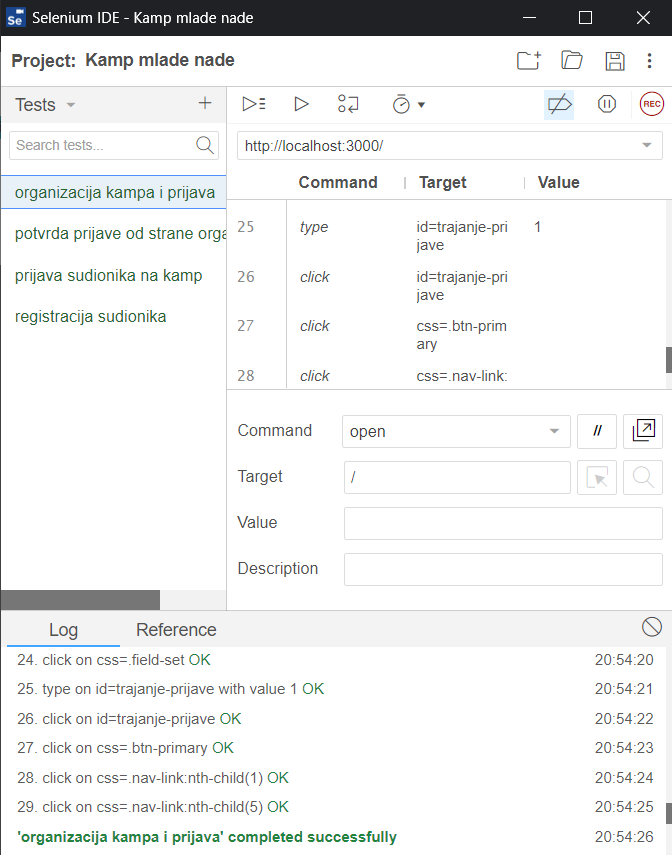
\includegraphics[scale=0.6]{organizacijaKampaIPrijava}
				\caption{Organizacija kampa i prijava}
			\end{figure}
			
			\clearpage
			
			\textbf{Ispitni slučaj 2: Prijava sudionika na kamp\\}
				\indent\textbf{Ulaz:}
					\begin{itemize}
						\item {Unos podataka korisnika u sklopu prijave za sudionika na kampu.}	
					\end{itemize}
				
				\textbf{Očekivani rezultat:}
					\begin{itemize}
						\item {Prijava evidentirana u bazi i samim tim se prikazuje organizatoru na stranici sa prijavama.}
					\end{itemize}
			
				{\textbf{Rezultat:} Očekivani rezultat je zadovoljen. Aplikacija je prošla test.\\}
			
			\begin{figure}[h]
				\centering
				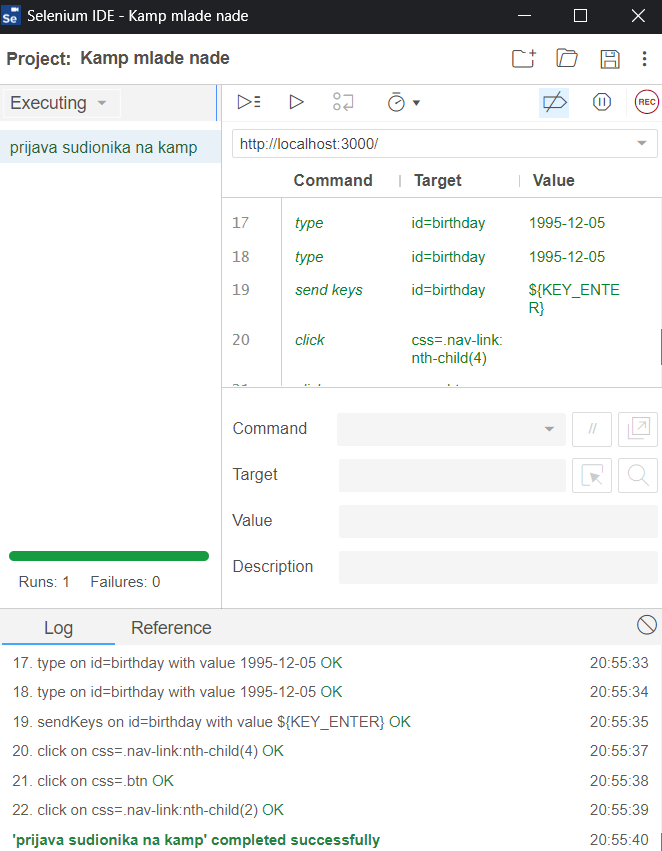
\includegraphics[scale=0.7]{prijavaSudionikaNaKamp}
				\caption{Organizacija kampa i prijava}
			\end{figure}
			
			\clearpage
			
			\textbf{Ispitni slučaj 3: Potvrda prijave od strane organizatora\\}
				\indent\textbf{Ulaz:}
					\begin{itemize}
						\item {Prijava korisnika u kojoj organizator vidi njegove podatke}
						\item {Odabir hoće li prihvatiti ili odbiti prijavu.}
					\end{itemize}
			
				\textbf{Očekivani rezultat:}
					\begin{itemize}
						\item {Na stranici na kojoj organizator inače može vidjeti prijave više nema prijave koja je potvrđena.}
						\item {Korisniku je poslan mail sa linkom i korisničkim imenom za registraciju.}
					\end{itemize}
			
				{\textbf{Rezultat:} Očekivani rezultat je zadovoljen. Aplikacija je prošla test.\\}
			
			\begin{figure}[h]
				\centering
				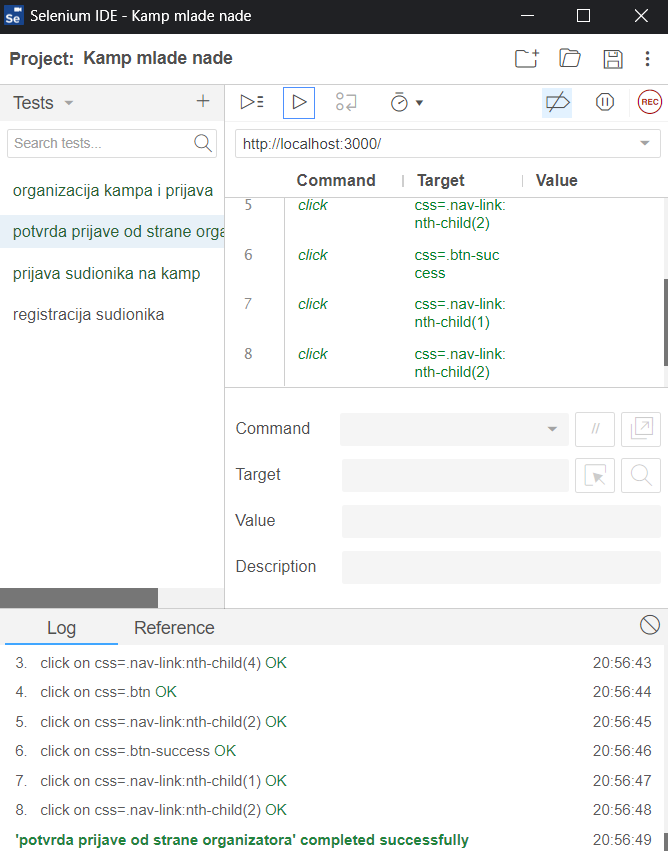
\includegraphics[scale=0.7]{potvrdaPrijaveOdStraneOrganizatora}
				\caption{Potvrda prijave od strane organizatora}
			\end{figure}

			
			\clearpage
			
			\textbf{Ispitni slučaj 4: Registracija sudionika\\}
			\indent\textbf{Ulaz:}
				\begin{itemize}
					\item {Web lokacija za kompletiranje registracije.}
					\item {Korisničko ime za registraciju.}
				\end{itemize}
			
			\textbf{Očekivani rezultat:}
				\begin{itemize}
					\item {Sudionik kampa uspješno se ulogirao.}
					\item {Sudionik kampa može vidjeti svoje korisničko ime u gornjem desnom kutu.}
					\item {Sudioniku se otvaraju opcije koje na web stranici ima svaki sudionik.}
				\end{itemize}
			
			{\textbf{Rezultat:} Očekivani rezultat je zadovoljen. Aplikacija je prošla test.\\}
			
			\begin{figure}[h]
				\centering
				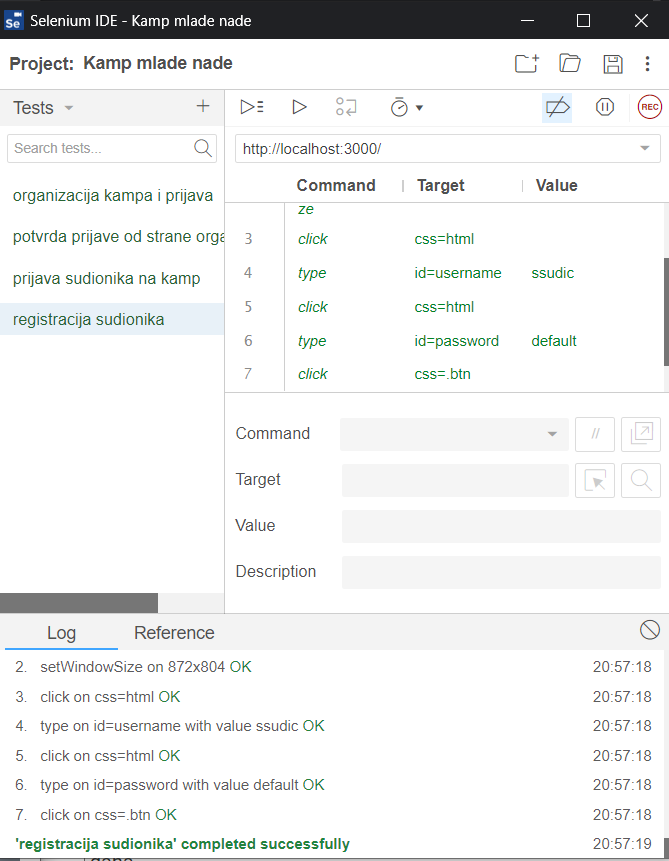
\includegraphics[scale=0.7]{registracijaSudionika}
				\caption{Registracija sudionika}
			\end{figure}
			
			\clearpage
			
			\textbf{Ispitni slučaj 5: Pokušaj organiziranja prijave nakon početka kampa\\}
			\indent\textbf{Ulaz:}
			\begin{itemize}
				\item {Datum i vrijeme početka kampa}
				\item {Odabir početka prijava u korisničkom sučelju.}
			\end{itemize}
			
			\textbf{Očekivani rezultat:}
			\begin{itemize}
				\item {Organiziranje prijave se odbija uz prikladnu poruku.}
				\item {Organizator je preusmjeren na početnu stranicu}
			\end{itemize}
			
			{\textbf{Rezultat:} Očekivani rezultat nije zadovoljen. Pokušajem organiziranja prijave nakon početka kampa događa se ReferenceError. Aplikacija nije prošla test.\\}
			
			\begin{figure}[h]
				\centering
				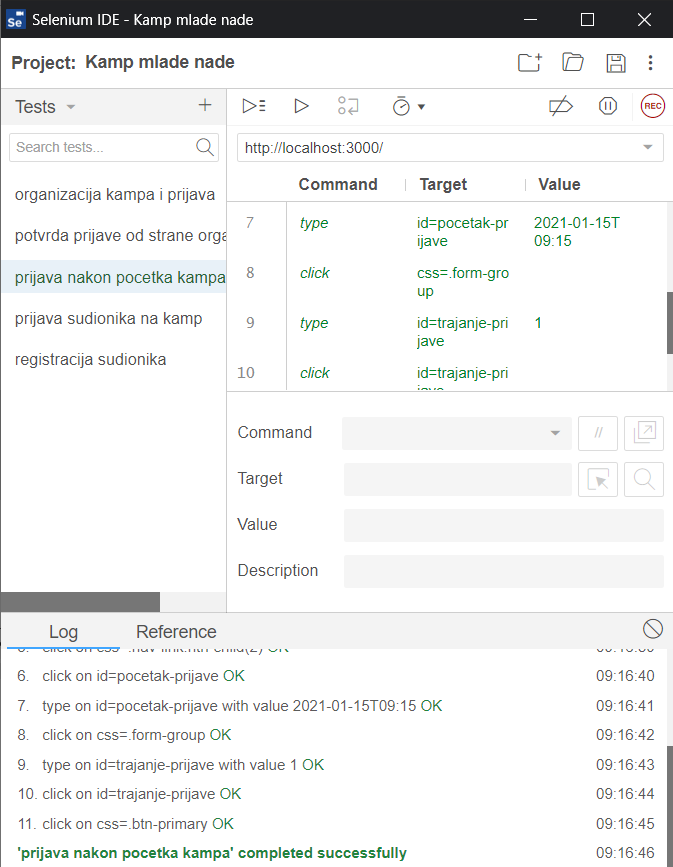
\includegraphics[scale=0.7]{prijavaNakonPocetka}
				\caption{Organiziranje prijave nakon početka kampa}
			\end{figure}

			
			\eject 
		
		
		\section{Dijagram razmještaja}
			
			Dijagrami razmještaja prikazuju računalne resurse potrebne za ispravno funkcioniranje sustava te njihove međusobne odnose: stvarne uređaje, komponente programske potpore koje se na njima izvršavaju i veze između njih. Dijagram razmještaja je statički strukturni UML-dijagram.\newline
			\indent Sustav je temeljen na arhitekturi \textit{klijent-poslužitelj}. Na poslužiteljskom računalu nalaze se web poslužitelj (na kojem se nalazi web aplikacija) i poslužitelj baze podataka (na kojem se nalazi baza podataka). Web poslužitelj i poslužitelj baze podataka su u vezi ovisnosti, točnije promjene na web poslužitelju uzrokuju promjene u bazi podataka. Na klijentskom se računalu nalazi web preglednik putem kojeg se pristupa web poslužitelju, odnosno web aplikaciji. Komunikacija između klijentskog i poslužiteljskog računala odvija se preko HTTP veze.\\\\
			
			\begin{figure}[htb]
				\centering
				\includegraphics[scale=0.7]{dijagrami/dijagramRazmještaja.PNG}
				\caption{Dijagram razmještaja}
				\label{fig: dijagram razmještaja}
			\end{figure}
			
			\eject 
		
		\section{Upute za puštanje u pogon}
		
			\subsection{Instalacija Git-a}
				Potrebno je instalirati Git korisničko sučelje prema uputama na stranici\footnote{\url{https://git-scm.com/book/en/v2/Getting-Started-Installing-Git}} i na računalu kreirati novu mapu za aplikaciju. Nakon instalacije potrebno je otvoriti \textit{Git Bash} i pozicionirati se u direktorij namijenjen za datoteke aplikacije. To se može učiniti tako da se desnim klikom na željenu mapu odabere opcija \textit{Git Bash Here}. Sljedeći korak je prijava ili registracija na sustav Gitlab putem internet stranice i postavljanje podataka o korisničkom računu na lokalni Git repozitorij. To se obavlja upisivanjem sljedećih naredbi u Git Bash:
					\begin{itemize}
						\item \textit{\textbf{git config user.email}} \textit{email}
						\item \textit{\textbf{git config user.name}} \textit{username}
					\end{itemize}
				U mapu je potrebno klonirati projekt odabirom opcije \textit{Clone} u gitlab repozitoriju te kopirati link ispod oznake \textit{Clone with HTTPS}. U Git Bash je potrebno upisati \textbf{\textit{git clone}} \textit{link}. Kod projekta je sada praćen u lokalnom Git repozitoriju.\\
				
				
			\subsection{Instalacija Heroku CLI-a}
				Heroku sučelje naredbenog retka (CLI) olakšava izradu i upravljanje Heroku aplikacijama izravno iz terminala. To je bitan dio upotrebe Herokua. Potrebno je preuzeti instalacijski paket\footnote{\url{https://devcenter.heroku.com/articles/heroku-cli}} minimalne verzije 7.0.x., pokrenuti instalacijski paket i slijediti upute na ekranu. Nakon instalacije potrebno je postaviti varijable okruženja sljedećim putem: \textit{Control Panel - System and Security - System - Advancded System Settings}. Otvorit će se prozor \textit{System properties} te je na kartici textit{Advanced} potrebno pritisnuti gumb \textit{Environment Variables}. U prozoru \textit{Environment Variables} u sekciji \textit{User Variables} potrebno je odabrati \textit{Path} i kliknuti gumb \textit{Edit}. U prozoru \textit{Edit environment variable} odabrati \textit{New} te upisati putanju do bin datoteke u folderu heroku, koja se najčešće nalazi u \textit{C://Program Files}. Ako je instalacija uspješna, u terminalu je moguće
				pokrenuti \textit{heroku -v} što će rezultirati prikazom verzije.\\
				
				
			\subsection{Kreiranje Heroku udaljenog repozitorija}
				Prvi je korak registracija i prijava u sustav Heroku. Nakon toga, potrebno je otvoriti terminal i pozicionirati se u git lokalni repozitorij, odnosno mapu kreiranu za projekt. Sljedeći korak je pokretanje naredbe \textbf{\textit{heroku login}} i nakon toga \textbf{\textit{heroku plugins:install java}}. Sljedeća naredba koju je potrebno pokrenuti je \textbf{\textit{heroku create}} u naredbenom retku (terminalu). Ta naredba stvara novu, praznu aplikaciju na Heroku poslužitelju povezanu s Git repozitorijem. Poželjno je nakon toga pokrenti naredbu \textbf{\textit{git remote -v}} što će rezultirati potvrdom da je udaljeni repozitorij pod imenom \textit{heroku} postavljen u aplikaciji.\newline
				\indent Potrebno je kreirati dvije aplikacije na Herokuu: jednu za backend i jednu za frontend. Jedna aplikacija je jedan poslužitelj.\\
				
				
			\subsection{Postavljanje baze podataka}
				Za postavljanje baze podataka potrebno je u kartici \textit{Resources} u postavkama aplikacije dodati \textit{Heroku Postgres} dodatak. Nakon ovog koraka na serveru će se konfigurirati prazna baza podataka. U kartici \textit{Settings} na postavkama baze podataka potrebno je odabrati opciju \textit{View Credentials}. Tada dobivamo podatke za spajanje na bazu koji su potrebni za konfiguraciju backenda.\\
				
				
			\subsection{Postavljanje backenda aplikacije na Heroku poslužitelj}
				Prije postavljanja backenda na poslužitelj potrebno je konfigurirati podatke za spajanje na bazu. U datoteci \textit{application.properties} unutar projekta potrebno je upisati podatke dobivene na sučelju Heroku. Nakon konfiguracije konekcije, potrebno je pokrenuti naredbu \textbf{\textit{maven install}}. Time će se izgraditi aplikacija. Unutar target direktorija unutar projekta kreirat će se \textit{.war} datoteka. Tu datoteku potrebno je prenijeti na Heroku poslužitelj.\newline
				\indent Koristeći naredbeni redak potrebno je postaviti se u direktorij projekta te pokrenuti naredbu \textbf{\textit{heroku war:deploy}} \textit{ime war datoteke} \textbf{\textit{–app}} \textit{naziv aplikacije kreirane na Heroku}. Nakon toga će na Heroku poslužitelj biti postavljen backend
				aplikacije.\\
				
				
			\subsection{Postavljanje frontenda aplikacije na Heroku poslužitelj}
				Nakon inicijalizacije udaljenog repozitorija na heroku, potrebno je pokrenuti naredbu \textbf{\textit{npm install}} za instalaciju svih paketa potrebnih \textit{node.j}-u.\newline
				\indent Da bi frontend aplikacije bio postavljen na Heroku poslužitelj, izvede se naredba
				\textbf{\textit{git push heroku master}} koja \textit{pusha} kod iz lokalnog repozitorija grane master na heroku udaljeni repozitorij. Ovu naredbu potrebno je pokrenuti svaki puta kada se želi postaviti novija verzija aplikacije na Heroku.
				\begin{figure}[htb]
					\centering
					
\includegraphics[scale=0.6]{slike/herokuPush.PNG}
					\caption{Postavljanje nove verzije aplikacije na Heroku}
					\label{fig: heroku}
				\end{figure}
			
				\indent Na kraju, naredba \textit{\textbf{heroku open}} služi za pokretanje aplikacije u pretpostavljenom pretraživaču.
			
			
			\eject 
	\chapter{Zaključak i budući rad}

		Rad na ovom projektu u sklopu predmeta Programsko inženjerstvo pružio nam je bogato iskustvo, kako u organizaciji rada u timu, tako i u upotrebi brojnih alata koje smo koristili te samoj izradi web aplikacije. 
		Naš je zadatak bio u nekoliko mjeseci napraviti web aplikaciju kampa \textit{Mlade nade} namijenjenu organizatorima, kako bi im olakšali posao organizacije, ali i budućim sudionicima i animatorima, koji na ovaj način puno brže i lakše podnose prijave.\newline
		\indent Na samom početku prvog ciklusa bilo je potrebno opisati i razraditi projektni zadatak. Iako smo u ranoj fazi mislili da bi lakše bilo opisivati funkcionalnosti usputno, za vrijeme rada na aplikaciji, pokazalo se da je detaljna razrada funkcionalnosti prije same izrade bila ne samo korisna, nego i nužna za jednostavniju organizaciju i rad. Dijagrami i obrasci uporabe izrađeni u prvom ciklusu (dijagrami obrazaca uporabe, sekvencijski dijagrami, dijagrami razreda i baze podataka) bili su temelj za daljnji rad članova tima zaduženih za backend i frontend. Dobro izrađena dokumentacija pomogla nam je izbjeći nedoumice oko razvoja funkcionalnosti i olakšala raspodjelu posla među članovima tima. U prvoj fazi projekta neki od nas su se prvi puta susreli s korištenim alatima i programskim jezicima odabranima za rad. Savladali smo osnove korištenja sustava Git, LaTex i izradu dokumentacijskih dijagrama te prvi puta u praksi koristili bazu podataka.\newline
		\indent U drugoj fazi projekta naišli smo na veće izazove. Kako većina nas nije imala iskustva u radu s korištenim alatima, bili smo primorani samostalno učiti kako bismo ostvarili zadani cilj. Bilo je potrebno dokumentirati ostale UML dijagrame i napisati popratnu dokumentaciju kako bi korisnici mogli lakše koristiti našu aplikaciju i kako bismo olakšali rad na unapređenju iste.\newline
		\indent Naša komunikacija ostvarena je čestim sastancima i zajedničkim radom što se pokazalo vrlo efikasnim. Uvidjeli smo da je za rad u timu sastavljenom od ovako velikog broja članova nužna dobra komunikacija i informiranost svih članova grupe o napretku projekta. Shvatili smo važnost dobre organizacije u smislu raspodjele posla među članovima tima te vremena potrebnog da se zadaci izvrše. Da bi tim funkcionirao kao cjelina, jako je važno da svaki član tima odradi svoj dio posla savjesno i na vrijeme, kako bi se izbjegao nepotrebni angažman ostalih članova tima. Sva stečena iskustva i znanja koristit ćemo i nadograđivati u budućim projektima.
		
		\eject 
	\chapter*{Popis literature}
		\addcontentsline{toc}{chapter}{Popis literature}
		
		
		\begin{enumerate}
			
			
			\item  Programsko inženjerstvo, FER ZEMRIS, \url{http://www.fer.hr/predmet/proinz}
			
			\item  I. Sommerville, "Software engineering", 8th ed, Addison Wesley, 2007.
			
			\item  T.C.Lethbridge, R.Langaniere, "Object-Oriented Software Engineering", 2nd ed. McGraw-Hill, 2005.
			
			\item  I. Marsic, Software engineering book``, Department of Electrical and Computer Engineering, Rutgers University, \url{http://www.ece.rutgers.edu/~marsic/books/SE}
			
			\item  The Unified Modeling Language, \url{https://www.uml-diagrams.org/}
			
			\item  Astah Community, \url{http://astah.net/editions/uml-new}
		\end{enumerate}
	
	
	\begingroup
	\renewcommand*\listfigurename{Indeks slika i dijagrama}
	%\renewcommand*\listtablename{Indeks tablica}
	%\let\clearpage\relax
	\listoffigures
	%\vspace{10mm}
	%\listoftables
	\endgroup
	\addcontentsline{toc}{chapter}{Indeks slika i dijagrama}


	
	\eject 
		
	\chapter{Dodatak: Prikaz aktivnosti grupe}
\addcontentsline{toc}{chapter}{Dodatak: Prikaz aktivnosti grupe}

\section{Dnevnik sastajanja}


\begin{packed_enum}
	\item sastanak
	\begin{packed_item}
		\item Datum: 05. listopada 2020.
		\item Prisustvovali: K.Kovačević, M.Magdalenić, M.Palčić, Z.Rezo, I.Sabolić, I.Šokčević, F.Vučić
		\item Teme sastanka:
		\begin{packed_enum}
			\item prijedlozi mogućih vlastitih tema projekta
			\item rasprava o znanjima i vještinama\\
		\end{packed_enum}
	\end{packed_item}
	
	\item sastanak
	\begin{packed_item}
		\item Datum: 07. listopada 2020.
		\item Prisustvovali: K.Kovačević, M.Magdalenić, M.Palčić, Z.Rezo, I.Sabolić, I.Šokčević, F.Vučić
		\item Teme sastanka:
		\begin{packed_item}
			\item dogovor podjele posla
			\item uvod u projekt i organizaciju\\
		\end{packed_item}
	\end{packed_item}
	
	\item sastanak
	\begin{packed_item}
		\item Datum: 14. listopada 2020.
		\item Prisustvovali: K.Kovačević, M.Magdalenić, M.Palčić, Z.Rezo, I.Sabolić, I.Šokčević, F.Vučić, E.Vušak
		\item Teme sastanka:
		\begin{packed_item}
			\item sastanak s asistentom
			\item rasprava o dobivenom zadatku\\
		\end{packed_item}
	\end{packed_item}
	
	\item sastanak
	\begin{packed_item}
		\item Datum: 28. listopada 2020.
		\item Prisustvovali: K.Kovačević, M.Magdalenić, M.Palčić, Z.Rezo, I.Sabolić, I.Šokčević, F.Vučić
		\item Teme sastanka:
		\begin{packed_item}
			\item definiranje funkcionalnosti aplikacije
			\item rasprava o dizajnu aplikacije\\
		\end{packed_item}
	\end{packed_item}
	
	\item sastanak
	\begin{packed_item}
		\item Datum: 04. studenoga 2020.
		\item Prisustvovali: K.Kovačević, M.Magdalenić, M.Palčić, Z.Rezo, I.Sabolić, I.Šokčević, F.Vučić, E.Vušak
		\item Teme sastanka:
		\begin{packed_item}
			\item revizija napravljene dokumentacije
			\item tehnička pitanja\\
		\end{packed_item}
	\end{packed_item}
	
	\item sastanak
	\begin{packed_item}
		\item Datum: 11. studenoga 2020.
		\item Prisustvovali: K.Kovačević, M.Magdalenić, M.Palčić, Z.Rezo, I.Sabolić, I.Šokčević, F.Vučić, E.Vušak
		\item Teme sastanka:
		\begin{packed_item}
			\item demonstracija funkcionalnosti i dokumentacije\\
		\end{packed_item}
	\end{packed_item}
	
	\item sastanak
	\begin{packed_item}
		\item Datum: 16. prosinca 2020.
		\item Prisustvovali: K.Kovačević, M.Magdalenić, M.Palčić, Z.Rezo, I.Sabolić, I.Šokčević, F.Vučić
		\item Teme sastanka:
		\begin{packed_item}
			\item podjela novih zadataka\\
		\end{packed_item}
	\end{packed_item}
	
	\item sastanak
	\begin{packed_item}
		\item Datum: 08. siječnja 2021.
		\item Prisustvovali: K.Kovačević, M.Magdalenić, M.Palčić, Z.Rezo, I.Sabolić, I.Šokčević, F.Vučić, E.Vušak
		\item Teme sastanka:
		\begin{packed_item}
			\item  demonstracija funkcionalnosti
			\item  tehnička pitanja\\
		\end{packed_item}
	\end{packed_item}
	
	
\end{packed_enum}

\eject


\section{Tablica aktivnosti}



\begin{longtabu} to \textwidth {|X[7, l]|X[1, c]|X[1, c]|X[1, c]|X[1, c]|X[1, c]|X[1, c]|X[1, c]|}
	
	\cline{2-8} \multicolumn{1}{c|}{\textbf{}} &     \multicolumn{1}{c|}{\rotatebox{90}{\textbf{Ivan Sabolić }}} & \multicolumn{1}{c|}{\rotatebox{90}{\textbf{Martin Palčić }}} &	\multicolumn{1}{c|}{\rotatebox{90}{\textbf{Filip Vučić }}} &	\multicolumn{1}{c|}{\rotatebox{90}{\textbf{Zvonimir Petar Rezo }}} &
	\multicolumn{1}{c|}{\rotatebox{90}{\textbf{Ivana Šokčević }}} &
	\multicolumn{1}{c|}{\rotatebox{90}{\textbf{Maja Magdalenić }}} &	\multicolumn{1}{c|}{\rotatebox{90}{\textbf{Katarina Kovačević }}} \\ \hline 
	\endfirsthead
	
	
	\cline{2-8} \multicolumn{1}{c|}{\textbf{}} &     \multicolumn{1}{c|}{\rotatebox{90}{\textbf{Ivan Sabolić}}} & \multicolumn{1}{c|}{\rotatebox{90}{\textbf{Martin Palčić }}} &	\multicolumn{1}{c|}{\rotatebox{90}{\textbf{Filip Vučić }}} &
	\multicolumn{1}{c|}{\rotatebox{90}{\textbf{Zvonimir Petar Rezo }}} &	\multicolumn{1}{c|}{\rotatebox{90}{\textbf{Ivana Šokčević}}} &
	\multicolumn{1}{c|}{\rotatebox{90}{\textbf{Maja Magdalenić }}} &	\multicolumn{1}{c|}{\rotatebox{90}{\textbf{Katarina Kovačević }}} \\ \hline 
	\endhead
	
	
	\endfoot
	
	
	\endlastfoot
	
	Upravljanje projektom 		& 3 &  &  &  &  &  & \\ \hline
	Opis projektnog zadatka 	&  &  &  &  & 1 &  & \\ \hline
	
	Funkcionalni zahtjevi       &  &  &  &  &  & 1 & 1 \\ \hline
	Opis pojedinih obrazaca 	& 1 & 1 & 1 & 1 & 1 & 1 & 1 \\ \hline
	Dijagram obrazaca 			& 1 &  &  &  &  & 1 & 1 \\ \hline
	Sekvencijski dijagrami 		& 1 &  &  &  &  &  &  \\ \hline
	Opis ostalih zahtjeva 		&  &  &  &  & 1 &  &  \\ \hline
	
	Arhitektura i dizajn sustava	 &  &  &  &  & 1 &  &  \\ \hline
	Baza podataka				&  &  &  &  &  & 2 & 2  \\ \hline
	Dijagram razreda 			& 1 &  &  &  &  & 1 &   \\ \hline
	Dijagram stanja				&  &  &  &  &  & 1 & 1 \\ \hline
	Dijagram aktivnosti 		&  &  &  &  &  & 1 & 1 \\ \hline
	Dijagram komponenti			&  &  &  &  &  & 1 & 1 \\ \hline
	Korištene tehnologije i alati 		& 1 &  &  &  &  &  &  \\ \hline
	Ispitivanje programskog rješenja 	& 1 & 1 & 1 & 1 &  &  &  \\ \hline
	Dijagram razmještaja			&  &  &  &  & 1 &  &  \\ \hline
	Upute za puštanje u pogon 		&  &  &  &  & 1 &  &  \\ \hline 
	Dnevnik sastajanja 			&  &  &  &  & 1 & 1 &  \\ \hline
	Zaključak i budući rad 		&  &  &  &  & 1 &  &  \\  \hline
	Popis literature 			&  &  &  &  &  &  &  \\  \hline
	&  &  &  &  &  &  &  \\ \hline \hline
	
	{Izrada početne stranice} 				& 1 & 1 & 1 & 1 &  &  &  \\ \hline 
	{Izrada baze podataka} 		 			& 1 & 1 & 1 & 1 &  &  & \\ \hline 
	{Spajanje s bazom podataka} 							& 1 & 1 & 1 & 1 &  &  &  \\ \hline
	{Back end} 							& 1 & 1 & 1 & 1 &  &  &  \\  \hline
	
	
\end{longtabu}


\eject

\begin{figure}
	\section{Dijagrami pregleda promjena}
	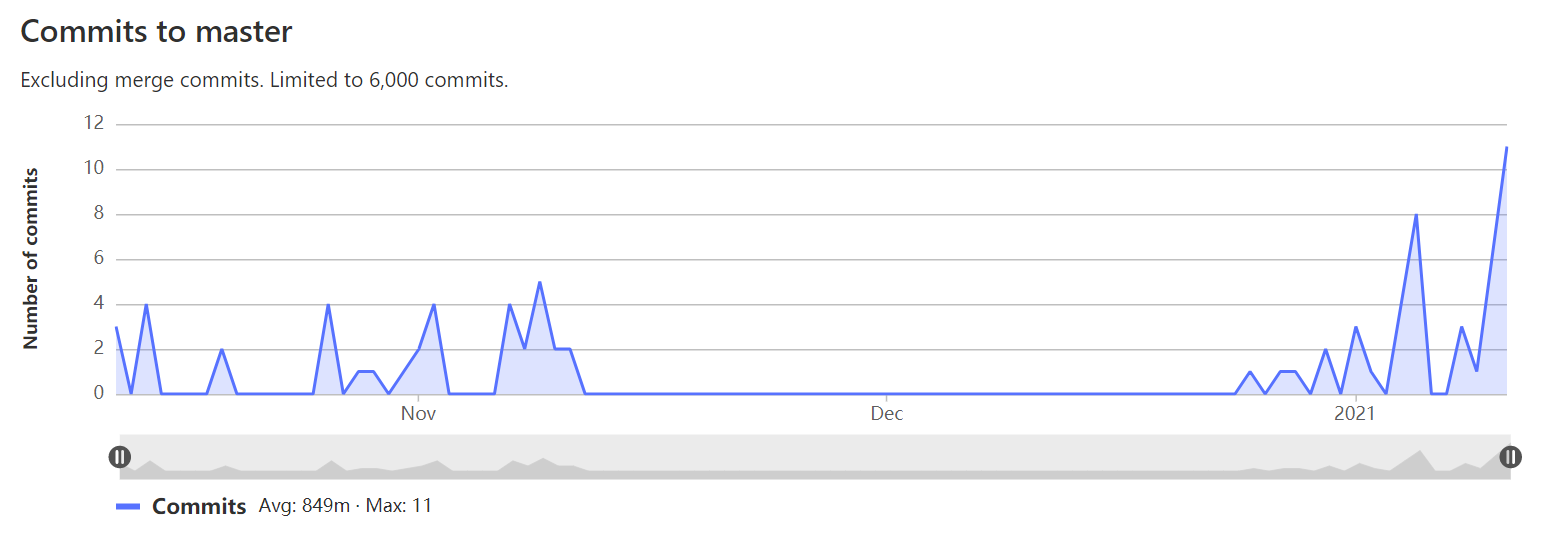
\includegraphics[scale=0.55]{slike/commitMaster.PNG}
	\newline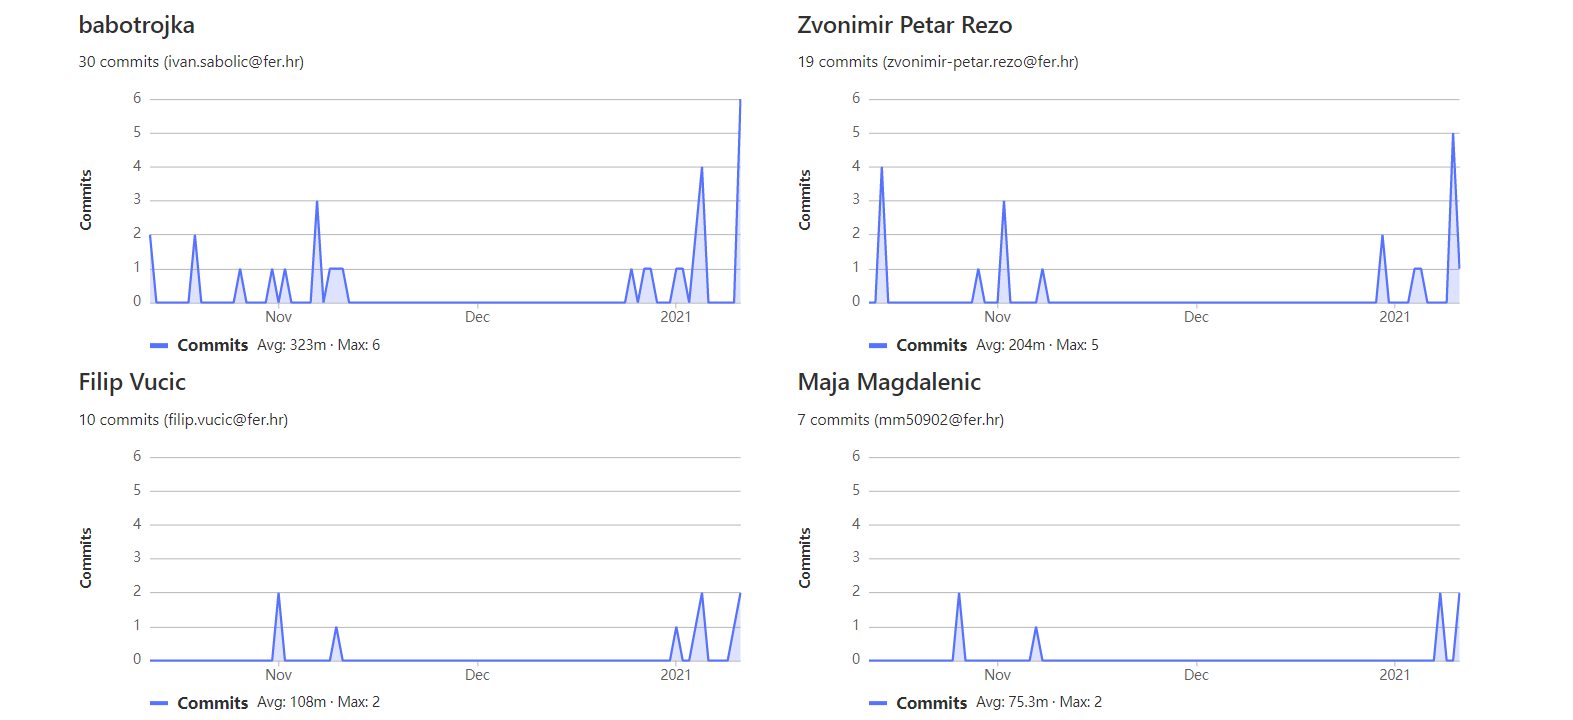
\includegraphics[scale=0.61]{slike/commitOsobe1.PNG}
	\newline
	\newline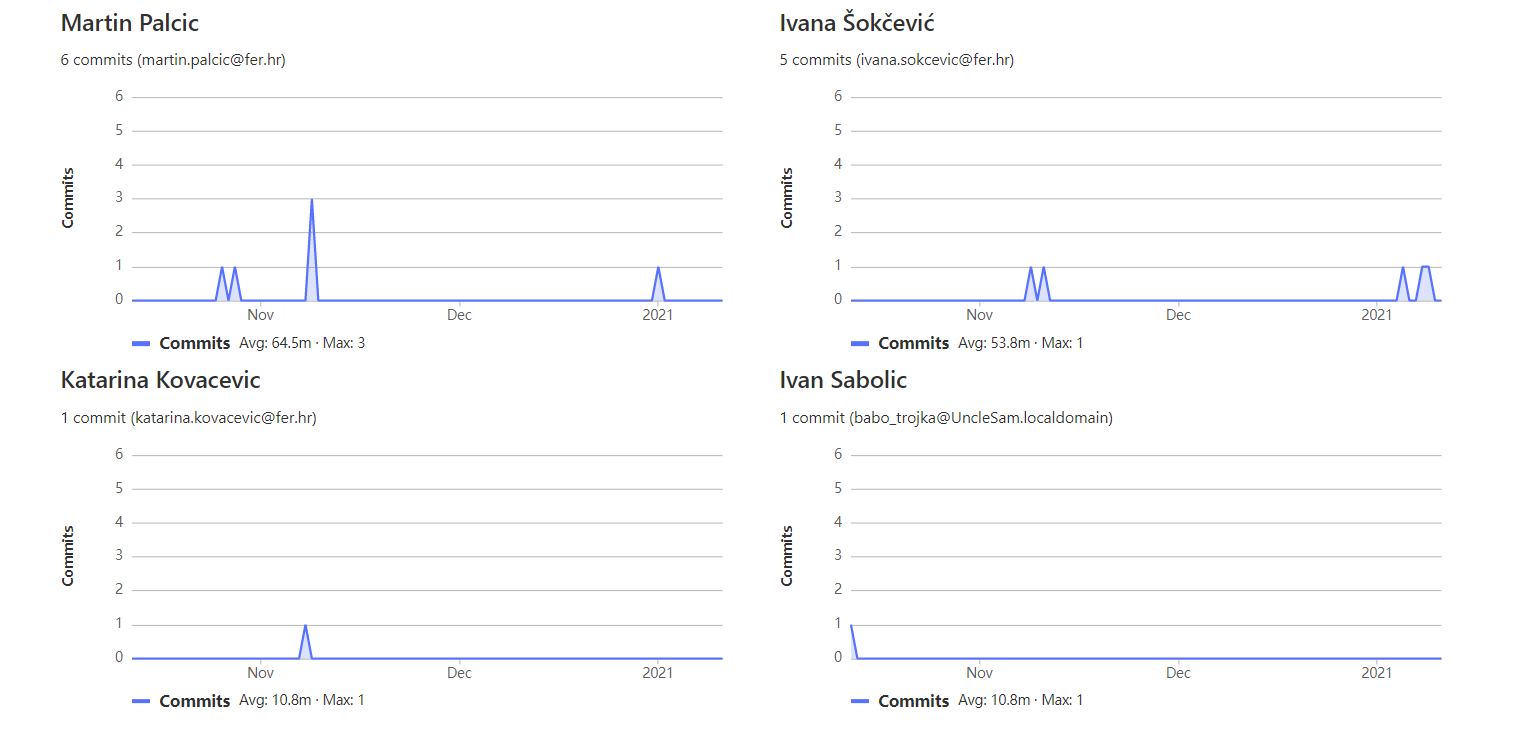
\includegraphics[scale=0.61]{slike/commitOsobe2.PNG}
\end{figure}



\end{document} %naredbe i tekst nakon ove naredbe ne ulaze u izgrađen dokument 


